\documentclass[a4paper,oneside,12pt]{report}
% Package yang diperlukan
\usepackage{fontspec}       % Font sistem untuk XeLaTeX/LuaLaTeX
\usepackage{setspace}       % Pengaturan jarak antarbaris
\usepackage{graphicx}      % Untuk memasukkan gambar
\usepackage{titling}       % Untuk kustomisasi halaman judul
\usepackage{geometry}      % Untuk mengatur margin halaman
\usepackage{listings}      % Untuk menampilkan blok kode
\usepackage{xcolor}        % Untuk menggunakan warna
\usepackage{float}         % Untuk kontrol penempatan float (seperti gambar)
\usepackage{xurl}          % Untuk pemutusan tautan URL yang lebih baik
\usepackage{hyperref}      % Untuk membuat hyperlink (URL, referensi)
\usepackage{indentfirst}   % Untuk memberi indentasi pada paragraf pertama setiap seksi
\usepackage{url}           % Untuk format URL
\usepackage{fancyhdr}      % Untuk kustomisasi header dan footer
\usepackage{tocloft}       % Untuk kustomisasi Daftar Isi
\usepackage{bookmark}      % Untuk manajemen bookmark PDF yang lebih baik
\usepackage{amsmath}       % Untuk rumus matematika
\usepackage{amssymb}       % Untuk simbol matematika
\usepackage{booktabs}      % Untuk tabel yang lebih rapi
\usepackage{caption}
\usepackage{subcaption}    % Untuk tata letak gambar berdampingan
\usepackage{tabularx}      % Untuk tabel dengan lebar otomatis sesuai margin
\usepackage{array}         % Untuk kontrol kolom tabel
\usepackage{enumitem}      % Untuk kontrol kerapatan daftar
\usepackage[none]{hyphenat} % Nonaktifkan seluruh pemotongan kata bertanda hubung
\usepackage{microtype}     % Tipografi halus dan protrusion antislop

% Font dan spasi standar laporan praktikum
\setmainfont{Times New Roman}
\onehalfspacing

%======================================================================
% PENGATURAN GEOMETRI HALAMAN
%======================================================================
\geometry{left=3cm, right=2.5cm, top=2cm, bottom=2.5cm}
\sloppy
\tolerance=10000
\emergencystretch=3em
\hfuzz=1.5pt
\hbadness=10000
\hyphenpenalty=10000
\exhyphenpenalty=10000
\righthyphenmin=62
\lefthyphenmin=62

%======================================================================
% PENGATURAN WARNA UNTUK BLOK KODE
%======================================================================
\definecolor{codegreen}{rgb}{0,0.6,0}
\definecolor{codegray}{rgb}{0.5,0.5,0.5}
\definecolor{codepurple}{rgb}{0.58,0,0.82}
\definecolor{backcolour}{rgb}{0.95,0.95,0.92}
\definecolor{darkblue}{rgb}{0,0,0.6}

%======================================================================
% PENGATURAN BLOK KODE (LISTINGS)
%======================================================================
\lstdefinestyle{commonstyle}{
    backgroundcolor=\color{backcolour},
    breakatwhitespace=false,
    breaklines=true,
    captionpos=b,
    keepspaces=true,
    numbers=left,
    numbersep=5pt,
    showspaces=false,
    showstringspaces=false,
    showtabs=false,
    tabsize=2,
    frame=single,
    basicstyle=\ttfamily\scriptsize,
    numberstyle=\tiny\color{codegray},
    columns=flexible,
    postbreak=\mbox{\textcolor{red}{$\hookrightarrow$}\space},
    breakindent=0pt,
    breakautoindent=false
}
\lstdefinestyle{pythonstyle}{
    style=commonstyle,
    language=Python,
    commentstyle=\color{codegreen},
    keywordstyle=\color{darkblue},
    stringstyle=\color{codepurple},
    emph={import,from,class,def,for,while,if,else,elif,try,except,finally},
    emphstyle=\color{darkblue}
}

%======================================================================
% PENGATURAN LAIN-LAIN
%======================================================================
\newcommand{\customfbox}[1]{%
  \setlength{\fboxsep}{0pt}%
  \setlength{\fboxrule}{0.5pt}%
  \fcolorbox{black}{white}{#1}%
}
\renewcommand{\figurename}{Gambar}
\renewcommand{\thefigure}{\arabic{figure}}
\renewcommand{\tablename}{Tabel}
\renewcommand{\thetable}{\arabic{table}}
\renewcommand{\theequation}{\arabic{equation}}
\renewcommand{\lstlistingname}{Listing}
\AtBeginDocument{\renewcommand{\thelstlisting}{\arabic{lstlisting}}}
\counterwithout{figure}{chapter}
\counterwithout{table}{chapter}
\counterwithout{equation}{chapter}
\hypersetup{
    colorlinks=true,
    linkcolor=black,
    filecolor=black,
    urlcolor=black,
    citecolor=black,
    pdftitle={Laporan Praktikum Penambangan Data Pertemuan 7},
    pdfpagemode=FullScreen,
    breaklinks=true
}
\pagestyle{fancy}
\fancyhf{}
\fancyfoot[C]{\thepage}
\renewcommand{\headrulewidth}{0pt}
\fancypagestyle{plain}{
    \fancyhf{}
    \fancyfoot[C]{\thepage}
    \renewcommand{\headrulewidth}{0pt}
}
\renewcommand{\contentsname}{Daftar Isi}
\renewcommand{\bibname}{Daftar Pustaka}
\renewcommand{\thechapter}{}
\renewcommand{\chaptername}{}
\renewcommand{\thesection}{\arabic{chapter}.\arabic{section}}
\renewcommand{\thesubsection}{\thesection.\arabic{subsection}}
\setcounter{secnumdepth}{3}
\setcounter{tocdepth}{3}
\renewcommand{\cftchapdotsep}{\cftdotsep}
\renewcommand{\cftchapleader}{\cftdotfill{\cftchapdotsep}}
\setlength{\cftchapindent}{0em}
\setlength{\cftsecindent}{2em}
\setlength{\cftsubsecindent}{4em}
\setlength{\cftchapnumwidth}{0em}
\setlength{\cftsecnumwidth}{2.5em}
\setlength{\cftsubsecnumwidth}{3.2em}
\setlength{\cftbeforechapskip}{4pt}
\setlength{\cftbeforesecskip}{1.5pt}
\setlength{\cftbeforesubsecskip}{0.5pt}
\renewcommand{\cftchappresnum}{}
\renewcommand{\cftchapaftersnum}{}
\newcommand{\tocboldsection}[1]{%
  \protect\renewcommand{\protect\cftchapfont}{\protect\bfseries}%
  #1%
  \protect\renewcommand{\protect\cftchapfont}{}%
}

%======================================================================
% AWAL DOKUMEN
%======================================================================
\begin{document}

% Halaman Judul
\newgeometry{left=3cm, right=2.5cm, top=2.5cm, bottom=3cm}
\begin{titlingpage}
\begin{spacing}{1}
\begin{center}
\vspace*{0.2cm}
{\large \textbf{\MakeUppercase{Laporan Praktikum}}} \\[0.4cm]
{\large \textbf{\MakeUppercase{Praktikum Penambangan Data}}} \\[0.4cm]
{\large \textbf{\MakeUppercase{Pertemuan 7}}} \\[0.4cm]
{\large \textbf{\MakeUppercase{Imbalanced Dataset dan Feature Selection}}} \\[1.5cm]


\includegraphics[height=7cm]{images/UGM.png} \\[0.7cm]

{\normalsize \textbf{Disusun oleh:}} \\[0.4cm]
\begin{tabular}{@{}l l @{}}
  \textbf{Nama}           & : Hafidz Rizqullah Prasetya \\
  \textbf{NIM}            & : 24/535493/SV/24243 \\
  \textbf{Kelas}          & : PL5A1 \\
  \textbf{Dosen Pengampu} & : Dr. Imam Fahrurrozi, S.T., M.Cs.
\end{tabular} \\[1.2cm]

{\normalsize \textbf{PROGRAM STUDI D-IV}} \\[0.2cm]
{\normalsize \textbf{TEKNOLOGI REKAYASA PERANGKAT LUNAK}} \\[0.2cm]
{\normalsize \textbf{DEPARTEMEN TEKNIK ELEKTRO DAN INFORMATIKA}} \\[0.2cm]
{\normalsize \textbf{SEKOLAH VOKASI}} \\[0.2cm]
{\normalsize \textbf{UNIVERSITAS GADJAH MADA}} \\[0.2cm]
{\normalsize \textbf{YOGYAKARTA}} \\[0.2cm]
{\normalsize \textbf{2026}} \\[1.2cm]
\end{center}
\end{spacing}
\end{titlingpage}
\restoregeometry

\thispagestyle{empty}
\clearpage
\stepcounter{page}
\thispagestyle{empty}

% --- Daftar Isi ---
\addcontentsline{toc}{chapter}{Daftar Isi}
\begin{spacing}{0.92}
\tableofcontents
\end{spacing}
\clearpage

% Mengatur penomoran halaman menjadi arab dan mulai dari 3
\pagenumbering{arabic}
\setcounter{page}{3}

\chapter[Tujuan Praktikum]{Tujuan Praktikum}
Berdasarkan Modul Pertemuan 7 Praktikum Penambangan Data, tujuan praktikum ini adalah:
\begin{enumerate}[noitemsep, topsep=4pt, parsep=2pt]
   \item Mahasiswa memahami konsep \textit{imbalanced dataset} serta permasalahan yang muncul akibat ketidakseimbangan kelas dalam model \textit{machine learning}.
   \item Mahasiswa mampu menerapkan teknik \textit{balancing data} seperti \textit{Random Under-Sampling}, \textit{Random Over-Sampling}, SMOTE, dan ADASYN untuk menyeimbangkan distribusi kelas pada dataset.
   \item Mahasiswa memahami konsep dan metode \textit{feature selection} (\textit{filter}, \textit{wrapper}, \textit{embedded}) untuk memilih fitur yang paling relevan.
\end{enumerate}

\clearpage

\chapter{Dasar Teori}

\section{Imbalanced Class}
\textit{Imbalanced class} adalah kondisi ketika satu kelas pada suatu himpunan data memiliki jumlah sampel jauh lebih besar dibanding kelas lainnya. Kelas dengan sampel banyak disebut kelas mayoritas, sedangkan kelas dengan sampel sedikit disebut kelas minoritas. Ketidakseimbangan ini membuat algoritma klasifikasi standar cenderung memprediksi kelas mayoritas dan melewatkan kelas minoritas \cite{istiana2023}.

Yang lebih menentukan adalah kelas mana yang terabaikan. Pada kasus deteksi stroke, penipuan kartu kredit, atau kegagalan mesin, kelas minoritas justru menjadi kelas yang paling perlu dikenali. Model yang selalu menebak ``tidak berisiko'' bisa mencapai akurasi 95\% pada dataset stroke tanpa benar-benar belajar apa pun. Nilai \textit{recall} kelas minoritas pada kondisi seperti ini mendekati nol \cite{istiana2023}.

Penanganan ketidakseimbangan kelas bisa ditempuh lewat tiga jalur: memanipulasi data pada level sampel (\textit{resampling}), memodifikasi algoritma lewat pembobotan biaya (\textit{cost-sensitive learning}), atau menggabungkan keduanya. Gambar~\ref{fig:imbalance} memperlihatkan bentuk khas sebaran dua kelas yang tidak seimbang pada ruang dua fitur.

\begin{figure}[htbp]
\centering
\fbox{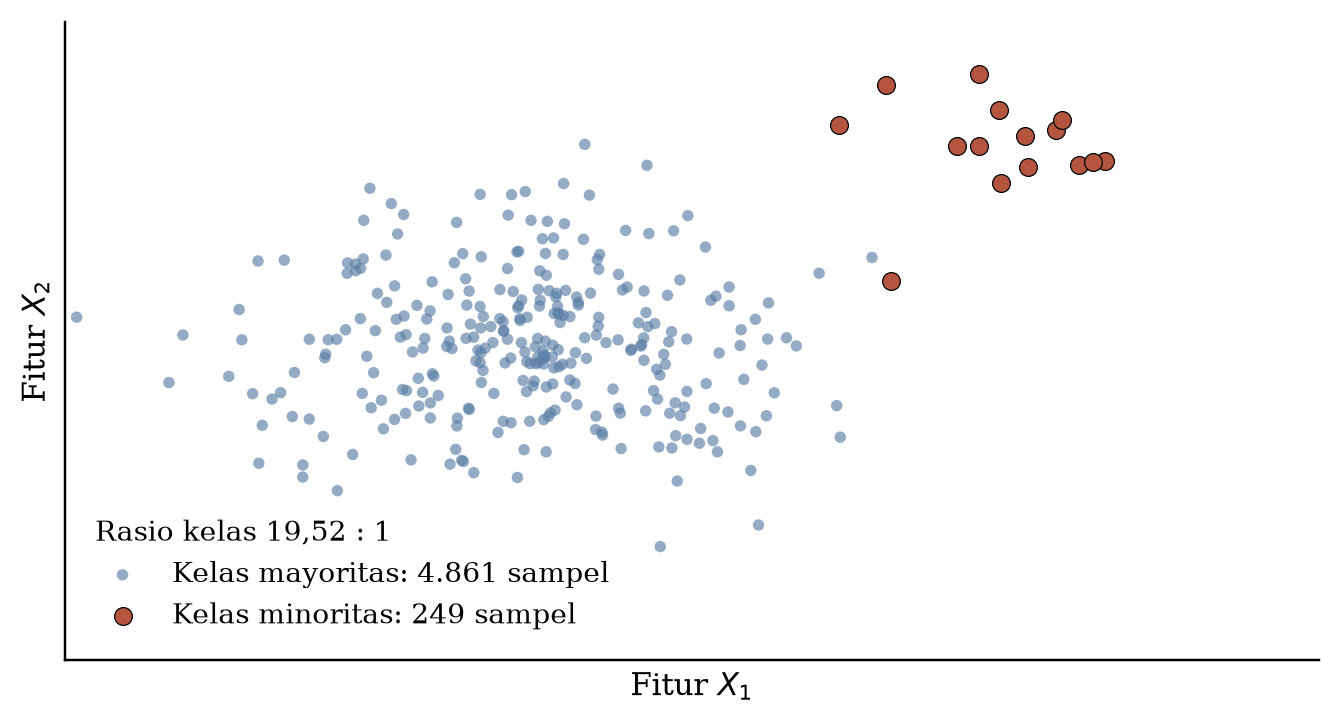
\includegraphics[width=0.78\textwidth]{images/gambar-imbalance.png}}
\caption{Ilustrasi ketidakseimbangan kelas pada ruang dua fitur. Kelas mayoritas memenuhi sebagian besar ruang, sedangkan kelas minoritas hanya menempati sebagian kecil area.}
\label{fig:imbalance}
\end{figure}

\section{Confusion Matrix}
\textit{Confusion matrix} adalah tabel kontingensi yang membandingkan label aktual dengan hasil prediksi model \cite{normawati2021}. Tabel~\ref{tab:confusion} memuat empat komponen dasarnya.

\begin{table}[htbp]
\centering
\caption{Susunan \textit{confusion matrix} untuk klasifikasi biner.}
\label{tab:confusion}
\begin{tabular}{|l|c|c|}
\hline
 & \textbf{Prediksi positif} & \textbf{Prediksi negatif} \\
\hline
\textbf{Aktual positif} & \textit{True Positive} (TP) & \textit{False Negative} (FN) \\
\hline
\textbf{Aktual negatif} & \textit{False Positive} (FP) & \textit{True Negative} (TN) \\
\hline
\end{tabular}
\end{table}

Keempat nilai tersebut menjadi dasar perhitungan metrik evaluasi:
\begin{align}
\mathit{Accuracy} &= \frac{TP + TN}{TP + TN + FP + FN} \\
\mathit{Precision} &= \frac{TP}{TP + FP} \\
\mathit{Recall} &= \frac{TP}{TP + FN} \\
\mathit{F1} &= \frac{2 \cdot \mathit{Precision} \cdot \mathit{Recall}}{\mathit{Precision} + \mathit{Recall}}
\end{align}

Pada data yang tidak seimbang, akurasi menjadi metrik yang menyesatkan. Prediksi yang selalu memilih kelas mayoritas tetap menghasilkan akurasi tinggi karena TN mendominasi perhitungan. \textit{Recall} dan \textit{F1-score} lebih menggambarkan kemampuan model mengenali kelas minoritas, sebab keduanya hanya menghitung TP terhadap jumlah sampel positif yang sebenarnya ada \cite{septiana2021}.

\section{Feature Selection}
\textit{Feature selection} adalah proses memilih subset fitur paling relevan dari seluruh fitur yang tersedia sebelum model dibangun \cite{pratama2023}. Ketika dimensi fitur terlalu besar, model rentan mengalami \textit{overfitting} dan waktu pelatihan naik tajam. Seleksi fitur memangkas dimensi ruang data dengan membuang fitur yang redundan atau tidak berhubungan dengan target \cite{guyon2003}.

Manfaatnya meliputi pengurangan waktu komputasi, peningkatan akurasi, dan pemahaman yang lebih baik atas model yang terbentuk. Tiga pendekatan yang umum dipakai dirangkum pada Tabel~\ref{tab:metode-fs}.

\begin{table}[htbp]
\centering
\caption{Perbandingan tiga pendekatan seleksi fitur.}
\label{tab:metode-fs}
\small
\begin{tabularx}{\linewidth}{|l|>{\raggedright\arraybackslash}X|>{\raggedright\arraybackslash}X|>{\raggedright\arraybackslash}X|}
\hline
\textbf{Pendekatan} & \textbf{Dasar penilaian} & \textbf{Biaya komputasi} & \textbf{Kekuatan} \\
\hline
\textit{Filter} & Statistik fitur terhadap target, tanpa melatih model & Ringan, satu kali hitung & Cepat dan mudah ditafsirkan \\
\hline
\textit{Wrapper} & Performa model pada setiap kombinasi fitur & Berat, model dilatih berulang & Menangkap interaksi antar-fitur \\
\hline
\textit{Embedded} & Seleksi berjalan di dalam proses pelatihan & Sedang & Seimbang antara akurasi dan waktu \\
\hline
\end{tabularx}
\end{table}

\section{Filter Method}
\textit{Filter method} mengevaluasi relevansi fitur dari sifat statistiknya terhadap variabel target, tanpa melibatkan model \textit{machine learning} \cite{guyon2003}. Ukuran yang lazim dipakai adalah korelasi Pearson atau Spearman, uji Chi-Square untuk fitur kategorikal, dan uji ANOVA untuk fitur numerik.

Uji ANOVA (\textit{Analysis of Variance}) membandingkan rata-rata suatu fitur antar-kelompok kelas. Nilai $F$ yang besar berarti rata-rata fitur tersebut berbeda nyata antar-kelas, sehingga fitur dinilai informatif untuk memisahkan kelas. Karena prosesnya hanya menghitung satu statistik per fitur, \textit{filter method} selesai dalam hitungan detik bahkan pada dataset berukuran besar.

\section{Wrapper Method}
\textit{Wrapper method} memakai algoritma \textit{machine learning} secara langsung sebagai fungsi penilai \cite{kohavi1997}. Metode ini mencoba berbagai kombinasi fitur, melatih model pada setiap kombinasi, lalu memilih kombinasi dengan performa terbaik. Tiga varian yang umum adalah \textit{Forward Selection} (menambah fitur satu per satu), \textit{Backward Elimination} (membuang fitur satu per satu), dan \textit{Recursive Feature Elimination} (RFE).

RFE bekerja dengan melatih model, mengurutkan fitur menurut besarnya bobot, membuang fitur dengan bobot terkecil, lalu mengulang proses tersebut sampai jumlah fitur yang tersisa sesuai target \cite{guyon2002}. Pendekatan ini lebih akurat dibanding \textit{filter} karena ikut memperhitungkan interaksi antar-fitur, tetapi biaya komputasinya jauh lebih besar sebab model dilatih berulang kali.

\section{Embedded Method}
\textit{Embedded method} menjalankan seleksi fitur bersamaan dengan proses pelatihan model. Contoh paling dikenal adalah regresi LASSO dengan regularisasi $L_1$ yang memaksa koefisien fitur tidak signifikan menjadi tepat nol \cite{tibshirani1996}, serta model berbasis pohon seperti \textit{Random Forest} dan \textit{Extra Trees} yang menghitung \textit{feature importance} dari penurunan \textit{impurity} pada setiap pemisahan node \cite{breiman2001}.

Pendekatan ini menggabungkan kelebihan dua metode sebelumnya: interaksi antar-fitur tetap diperhitungkan seperti \textit{wrapper}, sementara biaya komputasinya mendekati \textit{filter} karena seleksi menumpang pada satu kali pelatihan model.

\section{SMOTE}
\textit{Synthetic Minority Over-sampling Technique} (SMOTE) membangkitkan sampel minoritas baru, bukan menduplikasi sampel yang sudah ada \cite{chawla2002}. Untuk setiap sampel minoritas $a$, SMOTE mencari $k$ tetangga terdekat dari kelas yang sama (umumnya $k = 5$), memilih satu tetangga $b$ secara acak, lalu membuat sampel sintetis $c$ pada titik acak di sepanjang garis yang menghubungkan $a$ dan $b$:
\begin{equation}
c = a + \delta \, (b - a), \qquad \delta \sim U(0, 1)
\end{equation}

Karena titik sintetis lahir di antara sampel asli, kelas minoritas menjadi lebih rapat tanpa kehilangan informasi seperti pada \textit{under-sampling} \cite{wijayanti2021}. Gambar~\ref{fig:smote} menggambarkan proses tersebut.

\begin{figure}[htbp]
\centering
\fbox{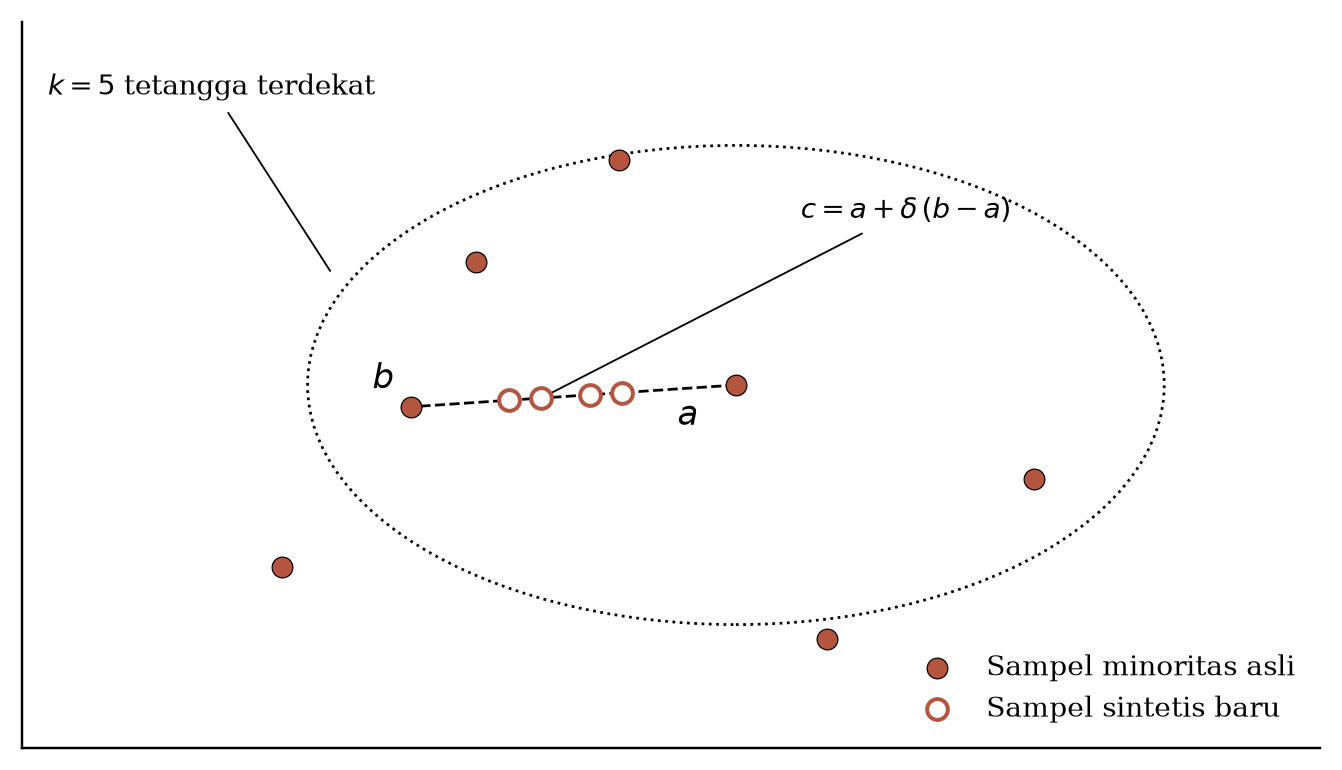
\includegraphics[width=0.78\textwidth]{images/gambar-smote.png}}
\caption{Cara kerja SMOTE. Sampel $a$ dipilih, lima tetangga terdekatnya ditandai, satu tetangga $b$ dipilih acak, lalu sampel sintetis $c$ dibangkitkan pada garis penghubung.}
\label{fig:smote}
\end{figure}

\section{ADASYN}
\textit{Adaptive Synthetic Sampling Approach} (ADASYN) adalah pengembangan SMOTE yang memperhitungkan tingkat kesulitan setiap sampel minoritas \cite{he2008}. ADASYN menghitung rasio $r_i = \Delta_i / K$ untuk setiap sampel minoritas, dengan $\Delta_i$ sebagai jumlah tetangga terdekat yang berasal dari kelas mayoritas. Rasio tersebut dinormalisasi menjadi $\hat{r}_i = r_i / \sum_i r_i$, lalu jumlah sampel sintetis yang dibangkitkan untuk sampel ke-$i$ adalah $g_i = \hat{r}_i \cdot G$, dengan $G$ sebagai total sampel sintetis yang dibutuhkan.

Akibatnya, sampel minoritas yang berada dekat batas keputusan menerima porsi sintetis lebih besar, sedangkan sampel di area yang mudah dipisahkan menerima porsi lebih kecil. Perbedaan ini yang membedakan ADASYN dari SMOTE yang memperlakukan semua sampel minoritas secara setara \cite{ramadhanti2022}.

\clearpage

\chapter{Alat dan Bahan}

Sesuai Modul Pertemuan 7 Praktikum Penambangan Data, alat dan bahan yang digunakan dalam praktikum ini meliputi:

\vspace{0.1cm}
\noindent\textbf{A. Perangkat Keras}
\begin{enumerate}[noitemsep, topsep=1pt, parsep=0pt]
    \item Laptop atau komputer personal (PC) dengan kapasitas memori minimal 4 GB RAM (direkomendasikan 8 GB atau lebih).
    \item Koneksi internet yang stabil untuk mengakses lingkungan komputasi daring dan mengunduh berkas dataset.
\end{enumerate}

\vspace{0.1cm}
\noindent\textbf{B. Perangkat Lunak}
\begin{enumerate}[noitemsep, topsep=1pt, parsep=0pt]
    \item Sistem operasi modern (Windows, macOS, atau Linux).
    \item Peramban web (Google Chrome, Mozilla Firefox, atau Microsoft Edge).
    \item Lingkungan pengembangan interaktif Python: Google Colaboratory dan Jupyter Notebook lokal.
    \item Bahasa pemrograman Python versi 3.8 ke atas \cite{python-docs}.
    \item Pustaka pemrograman Python:
    \begin{itemize}[noitemsep, topsep=1pt, parsep=0.5pt]
        \item \texttt{pandas} dan \texttt{numpy} untuk manipulasi data tabular dan operasi matriks numerik \cite{pandas-docs,numpy-docs}.
        \item \texttt{matplotlib.pyplot} dan \texttt{seaborn} untuk pembuatan grafik dua dimensi \cite{matplotlib-docs,seaborn-docs}.
        \item \texttt{scikit-learn} untuk pengkodean label, pemodelan pohon keputusan, seleksi fitur (\texttt{f\_classif}, \texttt{RFE}, \texttt{ExtraTreesClassifier}), dan metrik evaluasi \cite{sklearn-docs,pedregosa2011}.
        \item \texttt{imbalanced-learn} untuk penyeimbang kelas \texttt{RandomUnderSampler}, \texttt{RandomOverSampler}, \texttt{SMOTE}, dan \texttt{ADASYN} \cite{imblearn-docs,lemaitre2017}.
    \end{itemize}
\end{enumerate}

\vspace{0.1cm}
\noindent\textbf{C. Dataset}
\begin{enumerate}[noitemsep, topsep=1pt, parsep=0pt]
    \item \textit{Stroke Prediction Dataset} dengan 5.110 baris dan 12 kolom, dipakai pada percobaan penyeimbangan kelas \cite{kaggle-stroke}.
    \item \textit{Heart Attack Analysis and Prediction Dataset} dengan 303 baris dan 14 kolom, dipakai pada percobaan seleksi fitur \cite{kaggle-heart}.
    \item \textit{Wine Quality (red)} dengan 1.599 baris dan 12 kolom, dipakai pada Tugas 2 \cite{uci-wine,cortez2009}.
\end{enumerate}

\clearpage

\chapter[\texorpdfstring{\tocboldsection{Hasil dan Pembahasan}}{Hasil dan Pembahasan}]{Hasil dan Pembahasan}

\section{Percobaan Latihan Praktikum}
Percobaan latihan mengikuti sembilan langkah pada Modul Pertemuan 7, lalu dilanjutkan dengan praktik seleksi fitur dari materi kuliah pertemuan yang sama. Percobaan pertama memakai \textit{Stroke Prediction Dataset} untuk penyeimbangan kelas, sedangkan percobaan seleksi fitur memakai \textit{Heart Attack Analysis and Prediction Dataset}. Seluruh eksperimen dijalankan pada Jupyter Notebook lokal dengan Python 3 dan pustaka \texttt{imbalanced-learn} versi 0.14.

Notebook yang sama bisa dibuka dan dijalankan ulang secara interaktif melalui Google Colaboratory pada tautan berikut:

\begin{center}
\href{https://colab.research.google.com/github/hafidzrizqullahprasetya/PPD/blob/main/pertemuan-7/praktikum-7-imbalanced-feature-selection.ipynb}{\textcolor{blue}{\url{https://colab.research.google.com/github/hafidzrizqullahprasetya/PPD/blob/main/pertemuan-7/praktikum-7-imbalanced-feature-selection.ipynb}}} \cite{colab-notebook}
\end{center}

\subsection{Persiapan dan Impor Pustaka}
Tahap awal menginstal pustaka \texttt{imbalanced-learn} yang menyediakan empat teknik penyeimbangan kelas, lalu mengimpor pustaka manipulasi data, visualisasi, pemodelan, seleksi fitur, dan metrik evaluasi.

\begin{lstlisting}[style=pythonstyle,caption={Instalasi pustaka penyeimbang kelas.}]
%pip install -q imbalanced-learn
\end{lstlisting}

\begin{figure}[H]
\centering
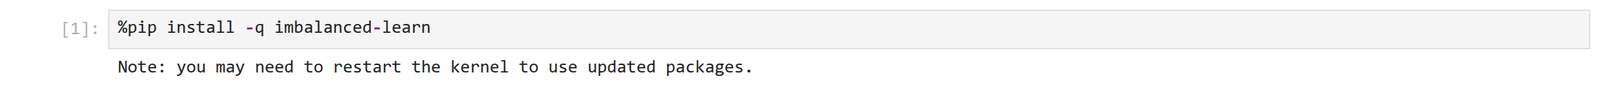
\includegraphics[width=0.9\textwidth]{images/ss-00-instalasi.png}
\caption{Tangkapan layar instalasi pustaka \texttt{imbalanced-learn} pada Jupyter Notebook.}
\label{fig:ss-instalasi}
\end{figure}

\begin{lstlisting}[style=pythonstyle,caption={Impor pustaka praktikum.}]
import numpy as np
import pandas as pd
import matplotlib.pyplot as plt
import seaborn as sns

from sklearn.model_selection import train_test_split
from sklearn.preprocessing import LabelEncoder
from sklearn.tree import DecisionTreeClassifier
from sklearn.ensemble import ExtraTreesClassifier, RandomForestClassifier
from sklearn.feature_selection import RFE, f_classif
from sklearn.metrics import accuracy_score, precision_score, recall_score, f1_score

from imblearn.under_sampling import RandomUnderSampler
from imblearn.over_sampling import RandomOverSampler, SMOTE, ADASYN

sns.set_theme(style="whitegrid")
pd.set_option("display.width", 130)
\end{lstlisting}

\begin{figure}[H]
\centering
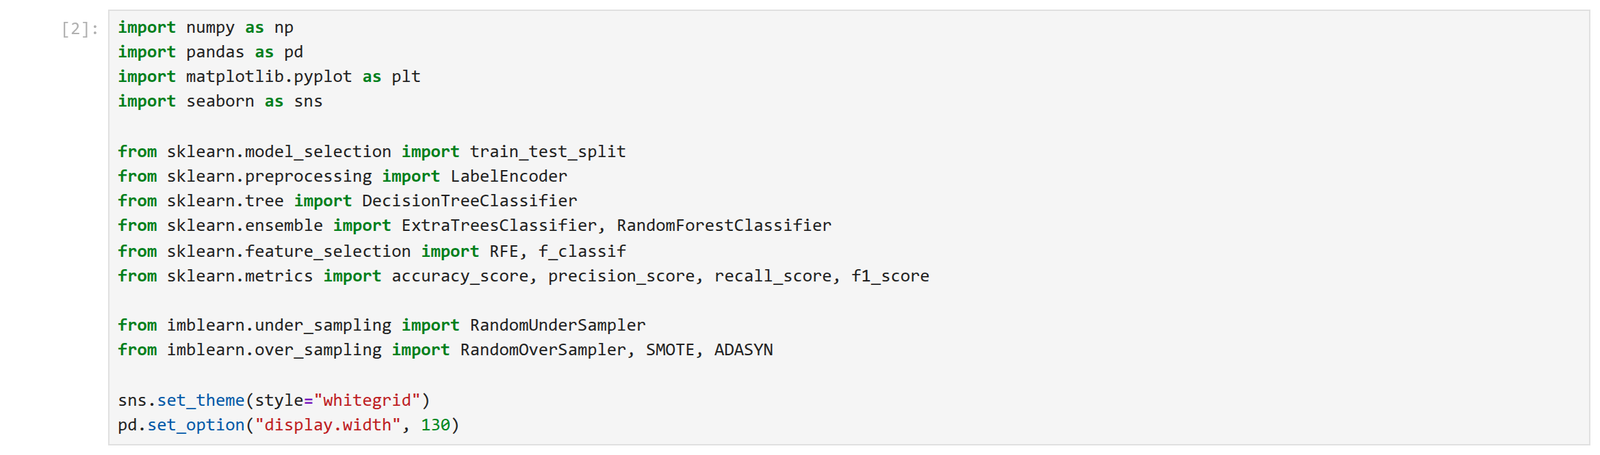
\includegraphics[width=0.9\textwidth]{images/ss-01-import-pustaka.png}
\caption{Tangkapan layar impor pustaka utama pada Jupyter Notebook.}
\label{fig:ss-import}
\end{figure}

\subsection{Memuat Stroke Prediction Dataset}
Dataset dibaca langsung dari repositori daring sehingga notebook dapat dijalankan ulang tanpa unggah berkas manual. Hasil pembacaan menunjukkan 5.110 baris dan 12 kolom.

\begin{lstlisting}[style=pythonstyle,caption={Membaca Stroke Prediction Dataset.}]
URL_STROKE = ("https://raw.githubusercontent.com/ganjar87/"
              "data_science_practice/main/healthcare-dataset-stroke-data.csv")
stroke = pd.read_csv(URL_STROKE)
print("Dimensi dataset:", stroke.shape)
stroke.head()
\end{lstlisting}

\begin{figure}[H]
\centering
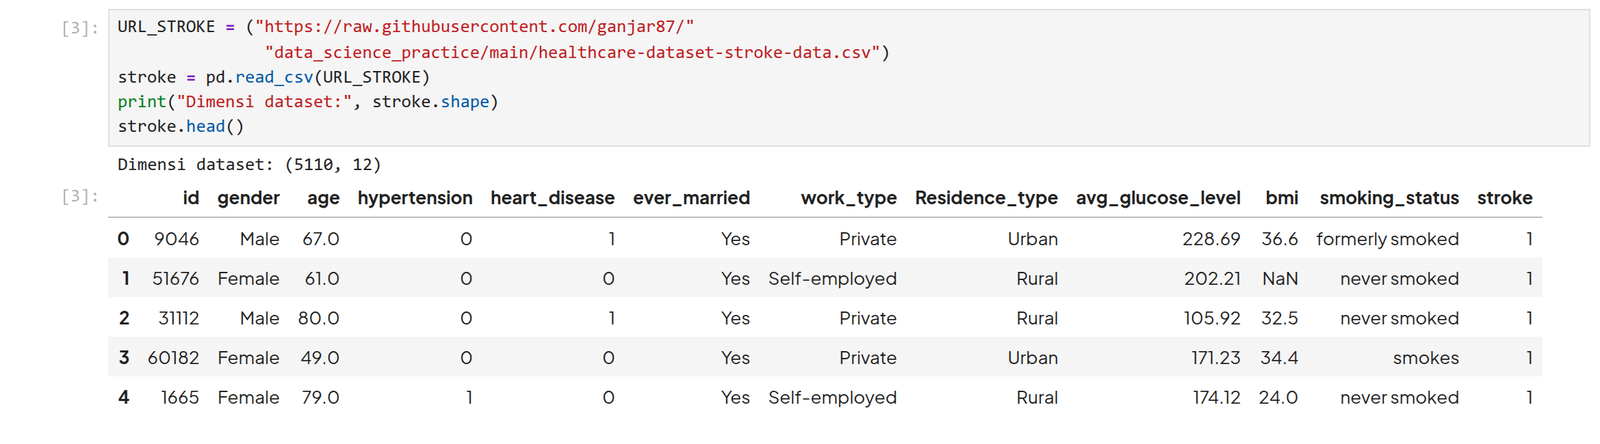
\includegraphics[width=0.9\textwidth]{images/ss-02-baca-dataset.png}
\caption{Tangkapan layar pembacaan data dan lima baris pertama dataset stroke.}
\label{fig:ss-baca}
\end{figure}

Pemeriksaan struktur data memakai \texttt{stroke.info()} memperlihatkan komposisi tipe data: empat kolom bilangan bulat, tiga kolom bilangan pecahan, dan lima kolom kategorikal bertipe teks. Kolom \texttt{bmi} tercatat hanya memiliki 4.909 nilai terisi dari 5.110 baris, tanda ada nilai kosong yang harus ditangani.

\begin{figure}[H]
\centering
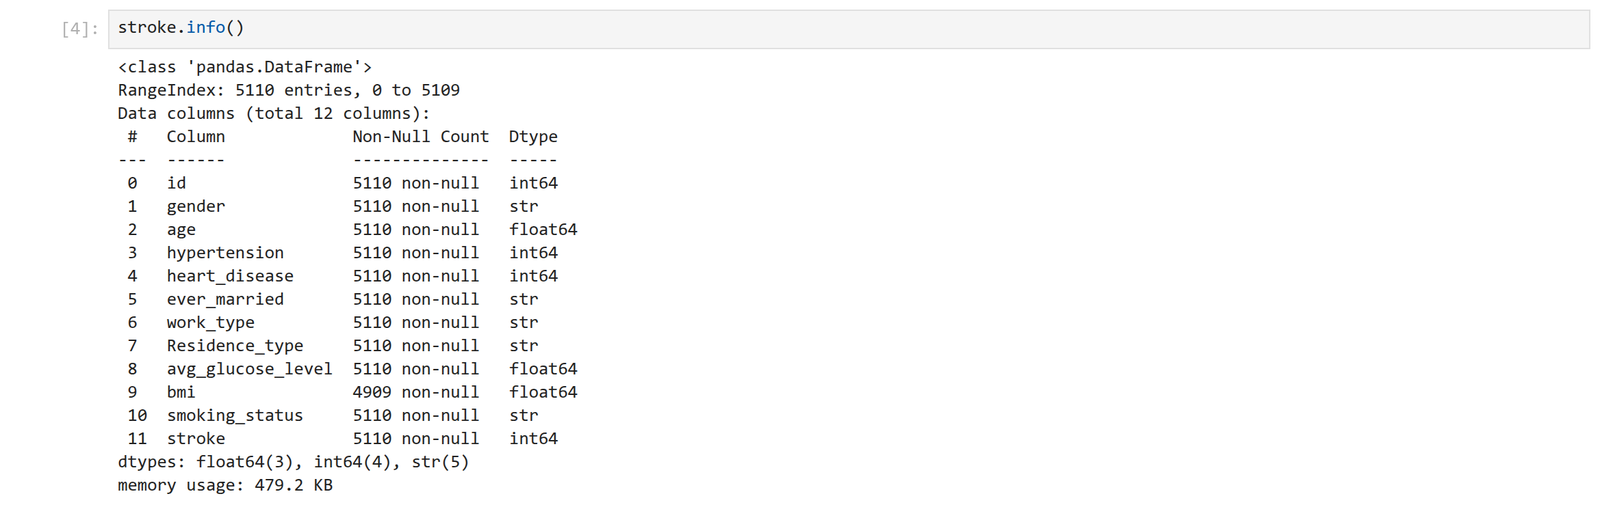
\includegraphics[width=0.9\textwidth]{images/ss-03-info-dataset.png}
\caption{Tangkapan layar struktur tipe data dan jumlah nilai terisi setiap kolom.}
\label{fig:ss-info}
\end{figure}

\subsection{Pemeriksaan Nilai Kosong}
Pemeriksaan nilai kosong memastikan kolom mana yang perlu diimputasi sebelum penyeimbangan dijalankan.

\begin{lstlisting}[style=pythonstyle,caption={Menghitung nilai kosong setiap kolom.}]
stroke.isnull().sum()
\end{lstlisting}

\begin{figure}[H]
\centering
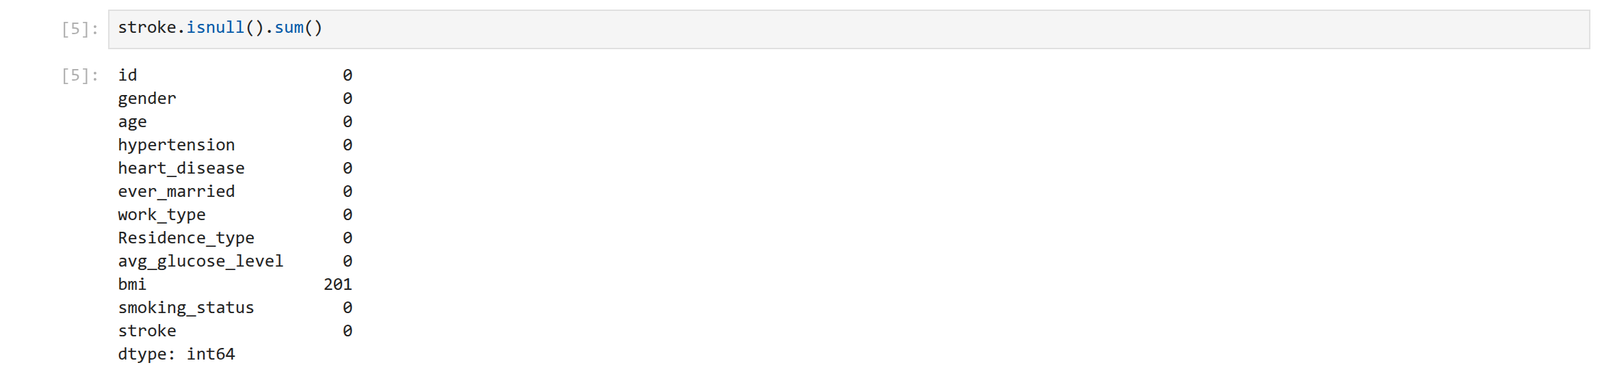
\includegraphics[width=0.45\textwidth]{images/ss-04-cek-null.png}
\caption{Tangkapan layar jumlah nilai kosong per kolom sebelum pembersihan.}
\label{fig:ss-null}
\end{figure}

Hasilnya hanya kolom \texttt{bmi} yang memiliki nilai kosong, sebanyak 201 baris. Sebelas kolom lain terisi penuh.

\subsection{Distribusi Kelas Target}
Proporsi kelas target dihitung dan digambarkan sebagai diagram lingkaran untuk melihat besarnya ketidakseimbangan.

\begin{lstlisting}[style=pythonstyle,caption={Menghitung proporsi kelas dan menggambar diagram lingkaran.}]
jumlah = stroke["stroke"].value_counts()
proporsi = stroke["stroke"].value_counts(normalize=True).mul(100).round(2)
print(pd.DataFrame({"jumlah": jumlah, "persen": proporsi}))

jumlah.plot(kind="pie", autopct="%.2f%%", labels=["Tidak stroke", "Stroke"], ylabel="")
plt.show()
\end{lstlisting}

\begin{figure}[H]
\centering
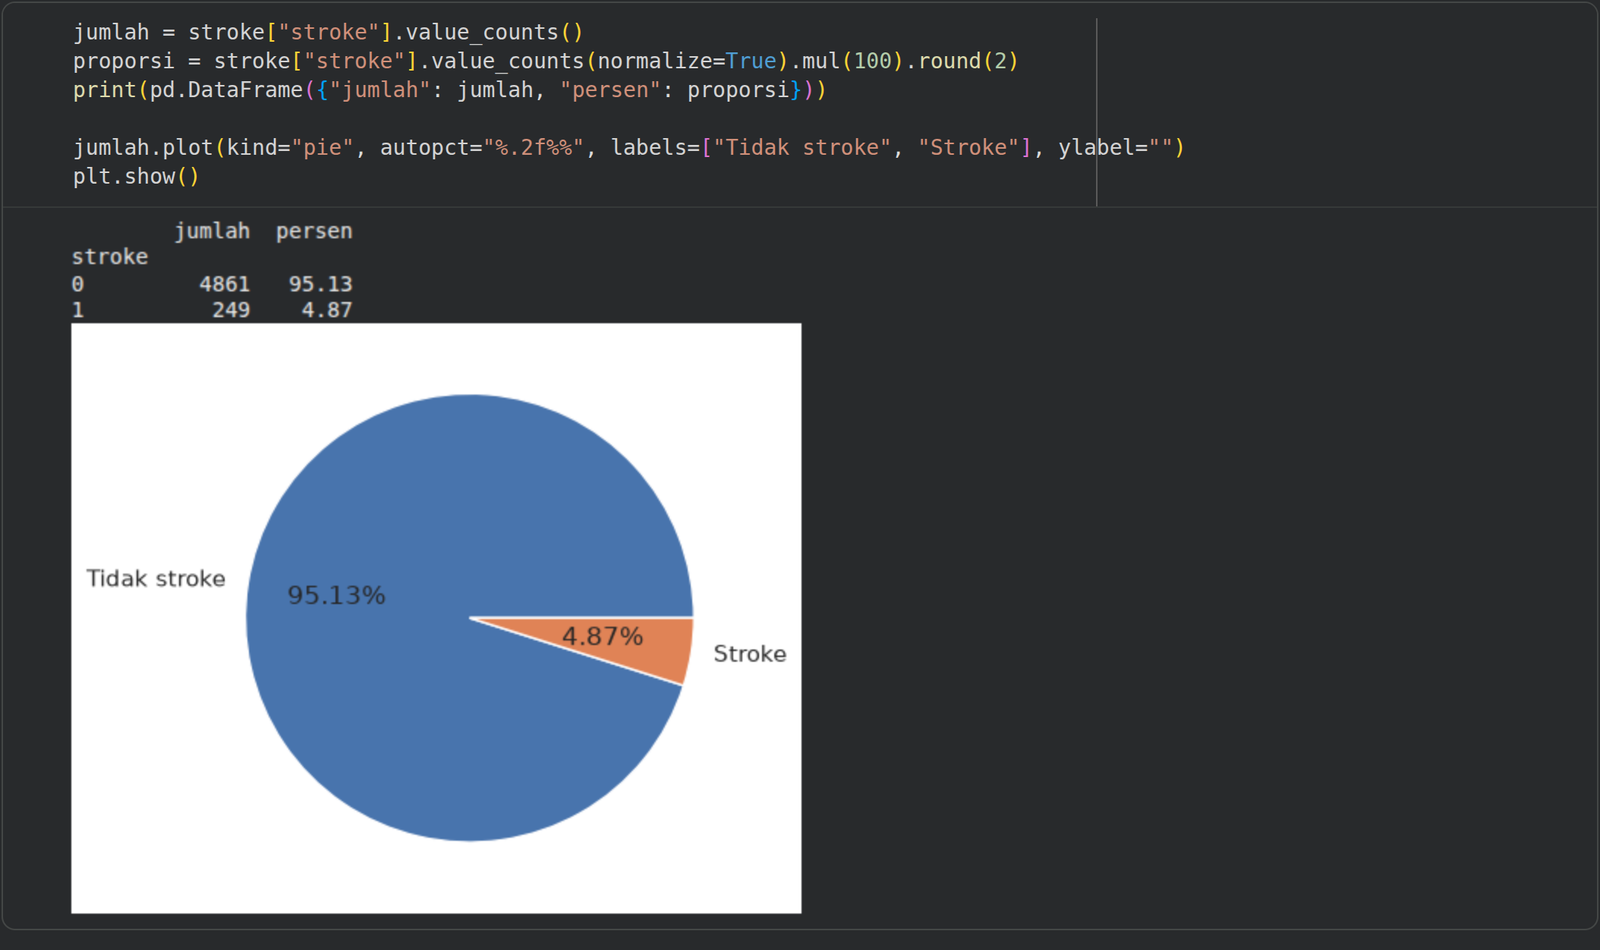
\includegraphics[width=0.85\textwidth]{images/ss-05-distribusi-kelas.png}
\caption{Tangkapan layar jumlah, persentase, dan diagram lingkaran distribusi kelas \texttt{stroke}.}
\label{fig:ss-distribusi}
\end{figure}

Dari 5.110 pasien, 4.861 di antaranya (95,13\%) tidak mengalami stroke dan hanya 249 pasien (4,87\%) yang mengalami stroke. Rasio kelas mayoritas terhadap kelas minoritas mencapai 19,52 banding 1. Angka ini menjelaskan mengapa penyeimbangan kelas diperlukan: model yang selalu menebak ``tidak stroke'' sudah mendapat akurasi 95,13\% tanpa mempelajari pola apa pun, sementara 249 pasien berisiko tinggi akan terlewat seluruhnya.

\subsection{Data Cleaning}
Nilai kosong pada kolom \texttt{bmi} diisi dengan rata-rata kolom tersebut. Pemilihan rata-rata didasarkan pada sifat BMI sebagai variabel kontinu dengan sebaran yang cukup simetris, sehingga nilai tengahnya mewakili populasi secara wajar. Setelah imputasi, pemeriksaan ulang memastikan tidak ada nilai kosong tersisa.

\begin{lstlisting}[style=pythonstyle,caption={Imputasi nilai kosong \texttt{bmi} dengan rata-rata.}]
stroke["bmi"] = stroke["bmi"].fillna(stroke["bmi"].mean())
stroke.isnull().sum()
\end{lstlisting}

\begin{figure}[H]
\centering
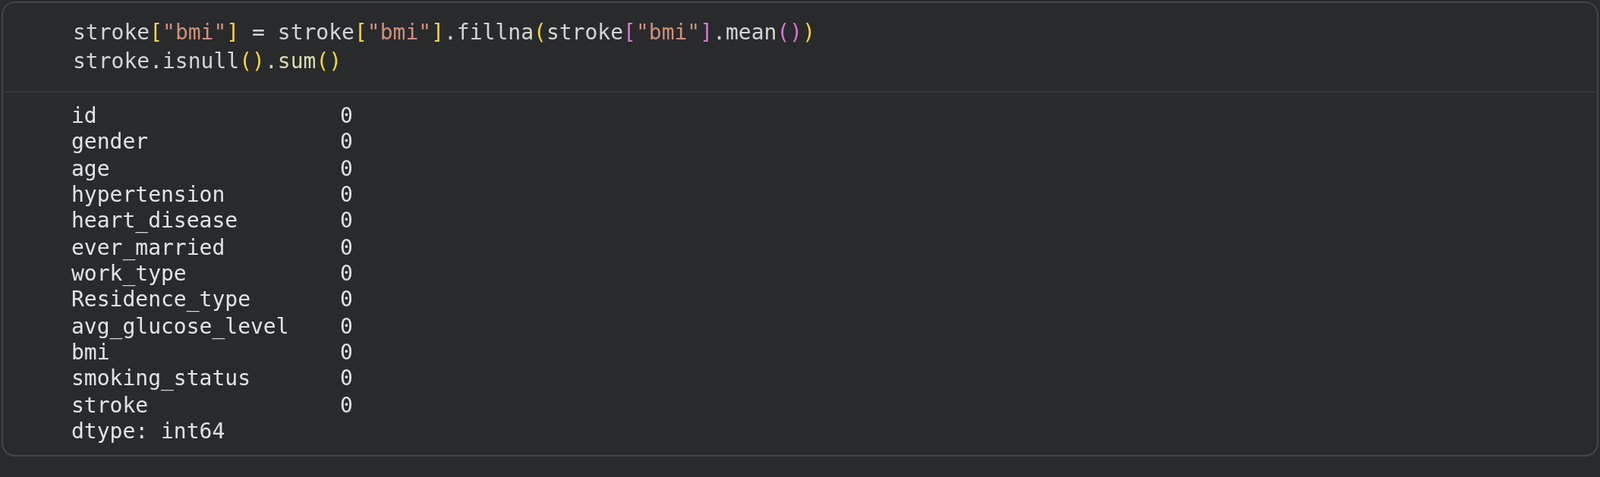
\includegraphics[width=0.45\textwidth]{images/ss-06-data-cleaning.png}
\caption{Tangkapan layar verifikasi data setelah imputasi. Seluruh kolom terisi penuh.}
\label{fig:ss-cleaning}
\end{figure}

\subsection{Pembagian Data dan Random Under-Sampling}
Fitur dipisahkan dari label target, fitur kategorikal dikodekan menjadi bilangan bulat dengan \texttt{LabelEncoder}, lalu data dibagi menjadi set pelatihan dan pengujian dengan rasio 75:25. Penyeimbangan hanya diterapkan pada set pelatihan. Set pengujian dibiarkan apa adanya agar evaluasi tetap mencerminkan sebaran asli di lapangan.

\begin{lstlisting}[style=pythonstyle,caption={Fungsi penyiapan data dan pembagian data latih-uji.}]
def siapkan_data(frame):
    fitur = frame.drop(columns=["id", "stroke"])
    target = frame["stroke"]
    encoder = LabelEncoder()
    for kolom in fitur.select_dtypes(exclude="number").columns:
        fitur[kolom] = encoder.fit_transform(fitur[kolom])
    return train_test_split(fitur.astype(float), target, test_size=0.25, random_state=42)


X_train, X_test, y_train, y_test = siapkan_data(stroke)
print("Latih:", X_train.shape, "| Uji:", X_test.shape)
print(pd.Series(y_train).value_counts())
\end{lstlisting}

\begin{figure}[H]
\centering
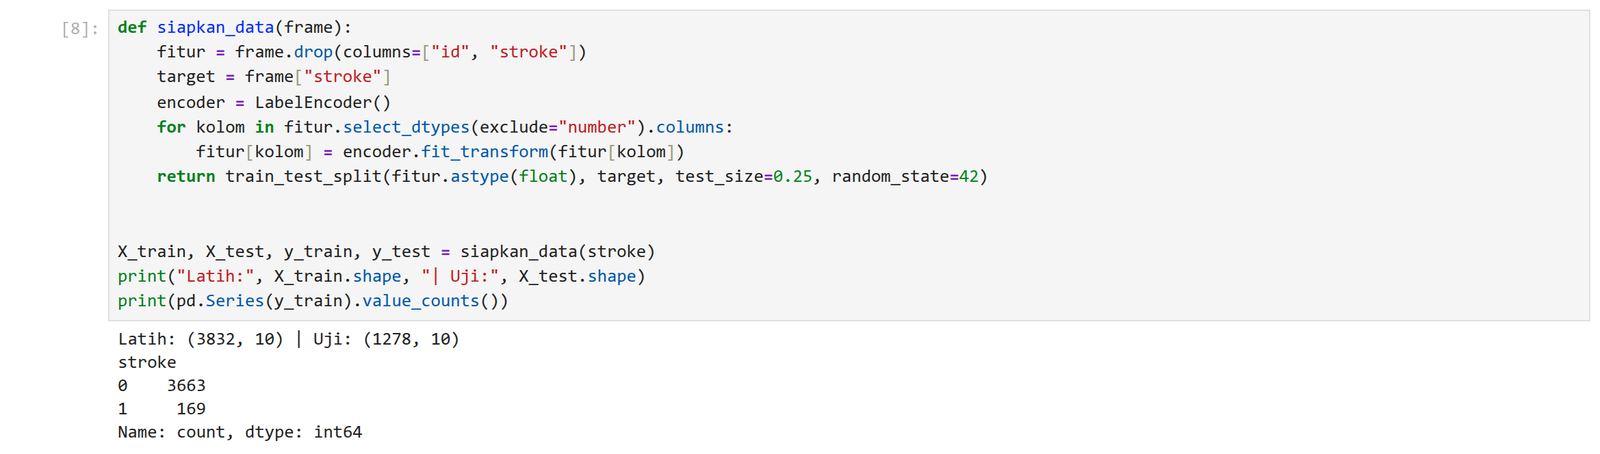
\includegraphics[width=0.9\textwidth]{images/ss-07-split-latih-uji.png}
\caption{Tangkapan layar dimensi set pelatihan, set pengujian, dan distribusi kelas pada set pelatihan.}
\label{fig:ss-split}
\end{figure}

Set pelatihan berisi 3.832 baris dengan komposisi 3.663 sampel kelas 0 dan 169 sampel kelas 1. Set pengujian berisi 1.278 baris.

\textit{Random Under-Sampling} memangkas sampel kelas mayoritas secara acak sampai jumlahnya setara dengan kelas minoritas.

\begin{lstlisting}[style=pythonstyle,caption={Penerapan \texttt{RandomUnderSampler} pada set pelatihan.}]
under = RandomUnderSampler(random_state=0)
X_under, y_under = under.fit_resample(X_train, y_train)
print("Sebelum:", pd.Series(y_train).value_counts().to_dict())
print("Sesudah:", pd.Series(y_under).value_counts().to_dict())
\end{lstlisting}

\begin{figure}[H]
\centering
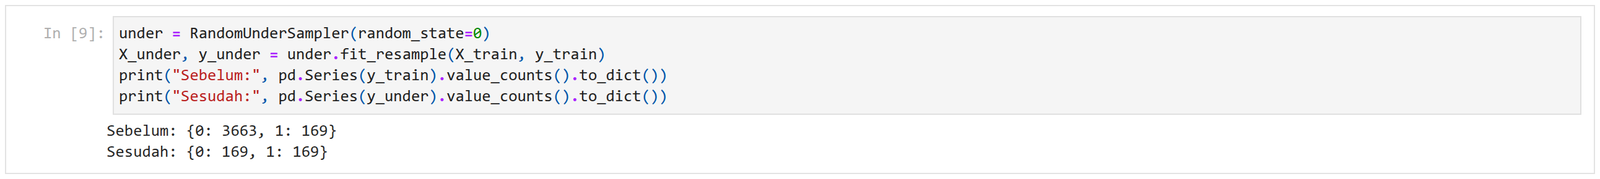
\includegraphics[width=0.7\textwidth]{images/ss-08-undersampling.png}
\caption{Tangkapan layar distribusi kelas sebelum dan sesudah \textit{Random Under-Sampling}.}
\label{fig:ss-rus}
\end{figure}

Kelas mayoritas turun dari 3.663 menjadi 169 sampel, sehingga set pelatihan hanya menyisakan 338 baris. Sebanyak 3.494 sampel mayoritas (95,4\% dari kelas tersebut) dibuang. Metode ini paling cepat, tetapi kehilangan informasi dalam jumlah besar berisiko menghapus pola yang sebenarnya penting.

\begin{figure}[H]
\centering
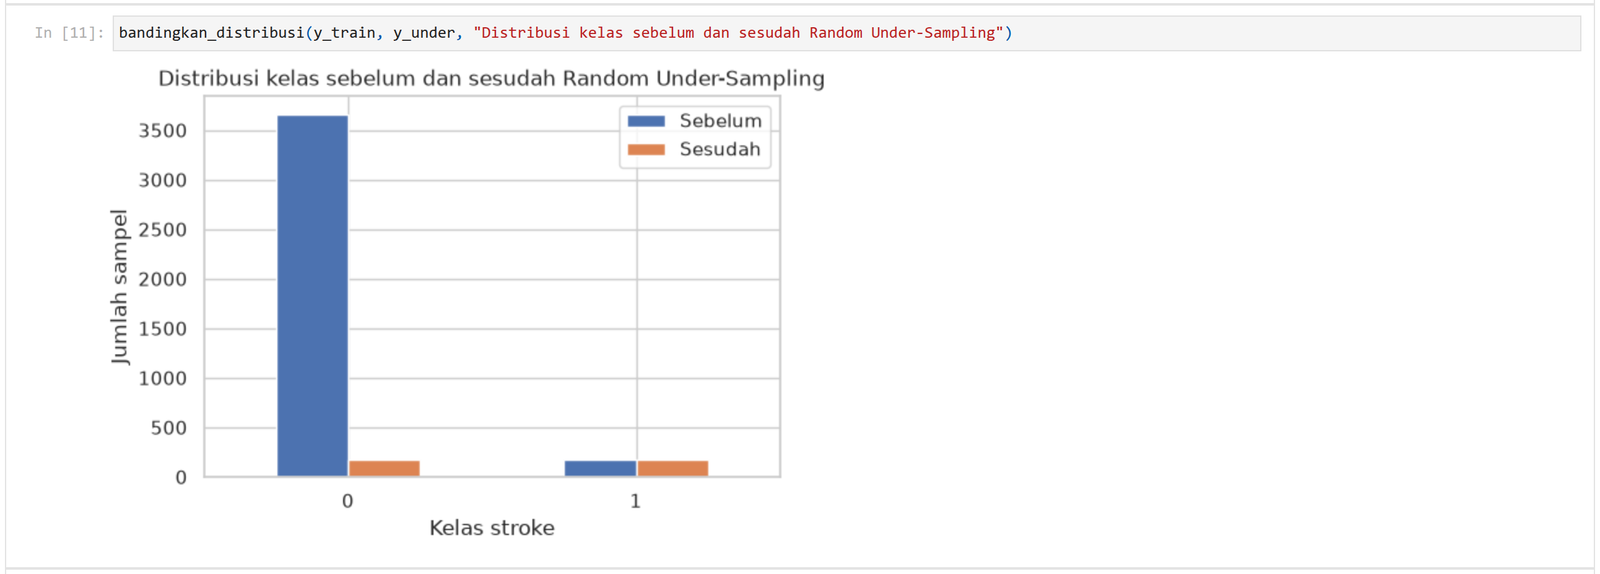
\includegraphics[width=0.68\textwidth]{images/ss-09-banding-undersampling.png}
\caption{Perbandingan jumlah sampel per kelas sebelum dan sesudah \textit{Random Under-Sampling}.}
\label{fig:ss-banding-rus}
\end{figure}

\begin{figure}[H]
\centering
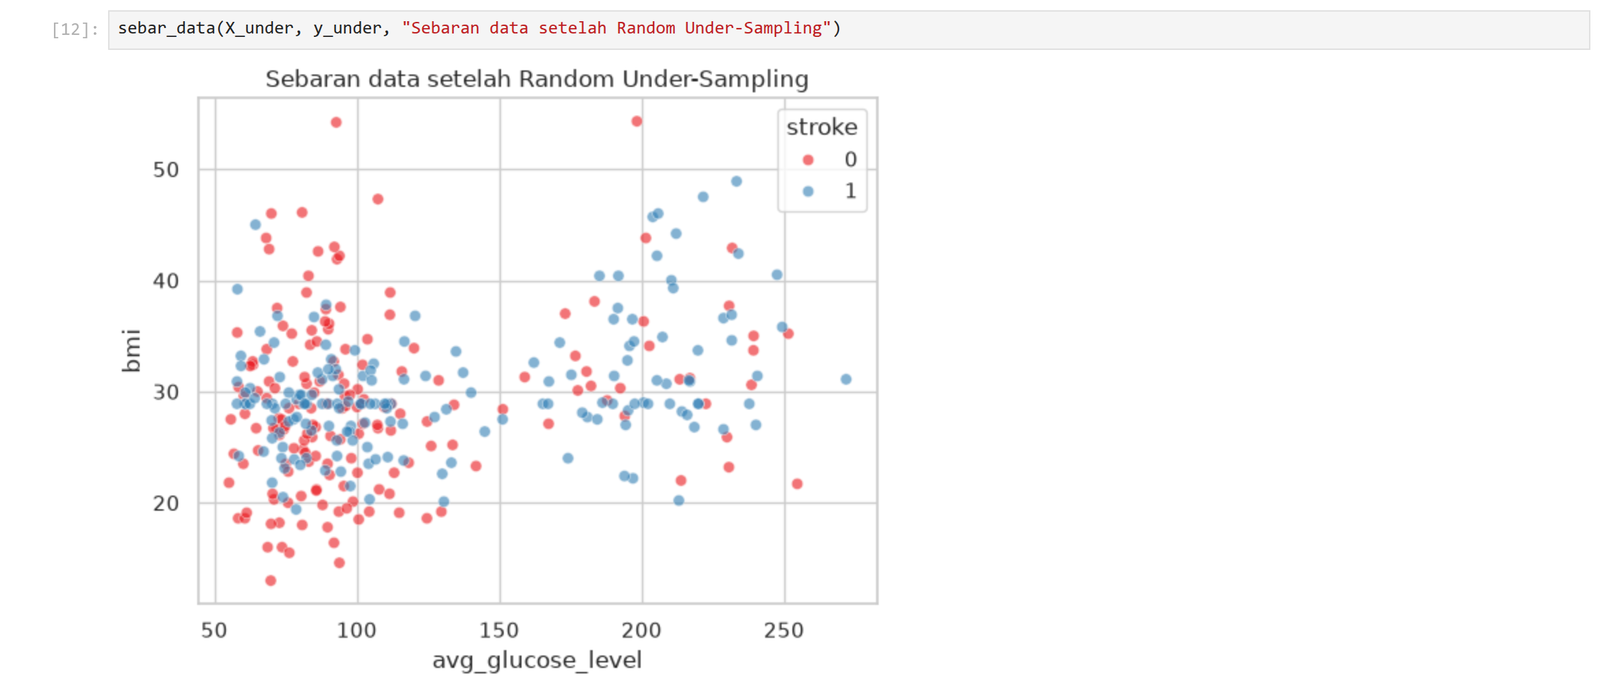
\includegraphics[width=0.68\textwidth]{images/ss-10-scatter-undersampling.png}
\caption{Sebaran data pada bidang \texttt{avg\_glucose\_level} dan \texttt{bmi} setelah \textit{Random Under-Sampling}. Titik kelas minoritas tidak lagi tenggelam di antara kelas mayoritas.}
\label{fig:ss-scatter-rus}
\end{figure}

\subsection{Random Over-Sampling}
\textit{Random Over-Sampling} menempuh arah sebaliknya: sampel kelas minoritas diduplikasi secara acak sampai jumlahnya menyamai kelas mayoritas.

\begin{lstlisting}[style=pythonstyle,caption={Penerapan \texttt{RandomOverSampler} pada set pelatihan.}]
over = RandomOverSampler(random_state=0)
X_over, y_over = over.fit_resample(X_train, y_train)
print("Sebelum:", pd.Series(y_train).value_counts().to_dict())
print("Sesudah:", pd.Series(y_over).value_counts().to_dict())
\end{lstlisting}

\begin{figure}[H]
\centering
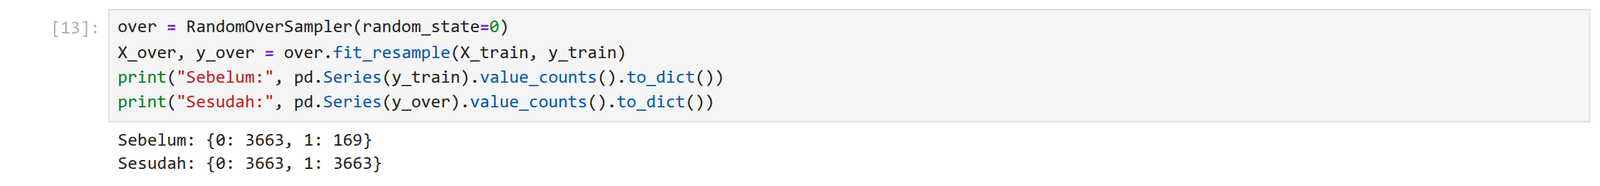
\includegraphics[width=0.7\textwidth]{images/ss-11-oversampling.png}
\caption{Tangkapan layar distribusi kelas sebelum dan sesudah \textit{Random Over-Sampling}.}
\label{fig:ss-ros}
\end{figure}

Kelas minoritas naik dari 169 menjadi 3.663 sampel, sehingga total set pelatihan menjadi 7.326 baris. Setiap sampel minoritas rata-rata terduplikasi 21,7 kali. Cara ini mempertahankan seluruh informasi asli, tetapi duplikasi berulang membuat model cenderung menghafal sampel yang sama dan memperbesar risiko \textit{overfitting}.

\begin{figure}[H]
\centering
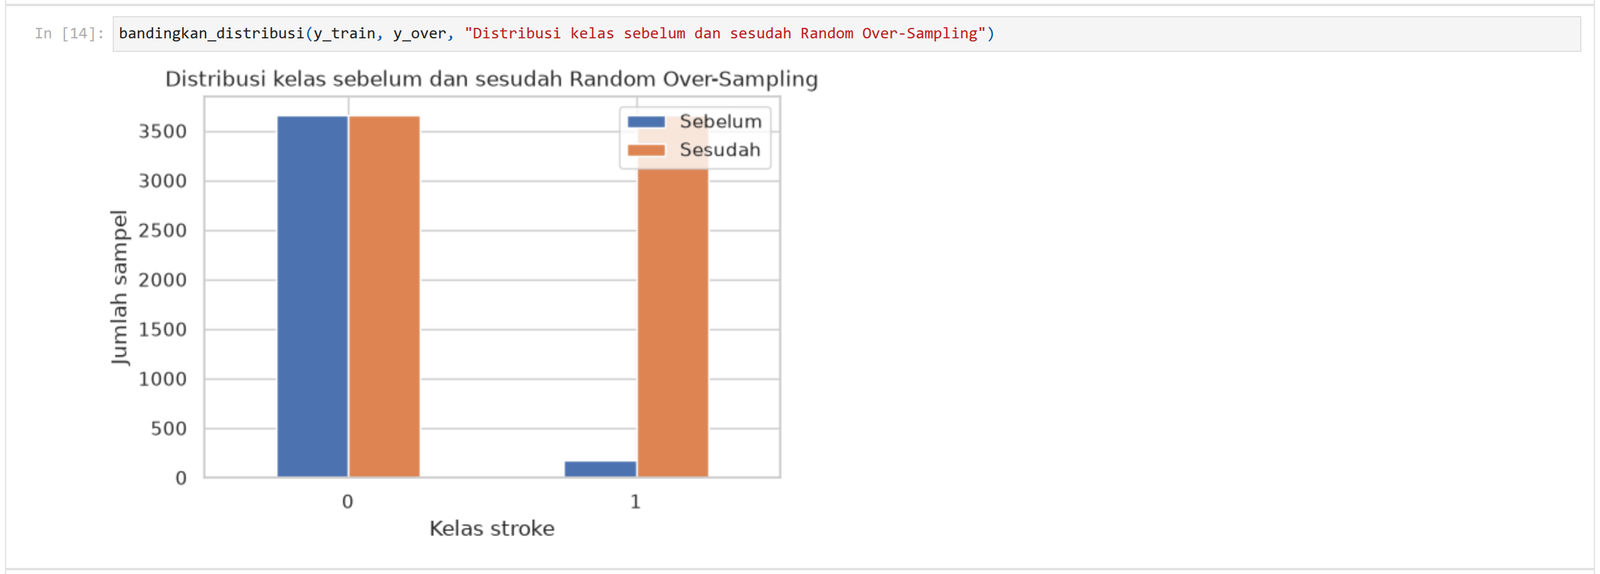
\includegraphics[width=0.68\textwidth]{images/ss-12-banding-oversampling.png}
\caption{Perbandingan jumlah sampel per kelas sebelum dan sesudah \textit{Random Over-Sampling}.}
\label{fig:ss-banding-ros}
\end{figure}

\begin{figure}[H]
\centering
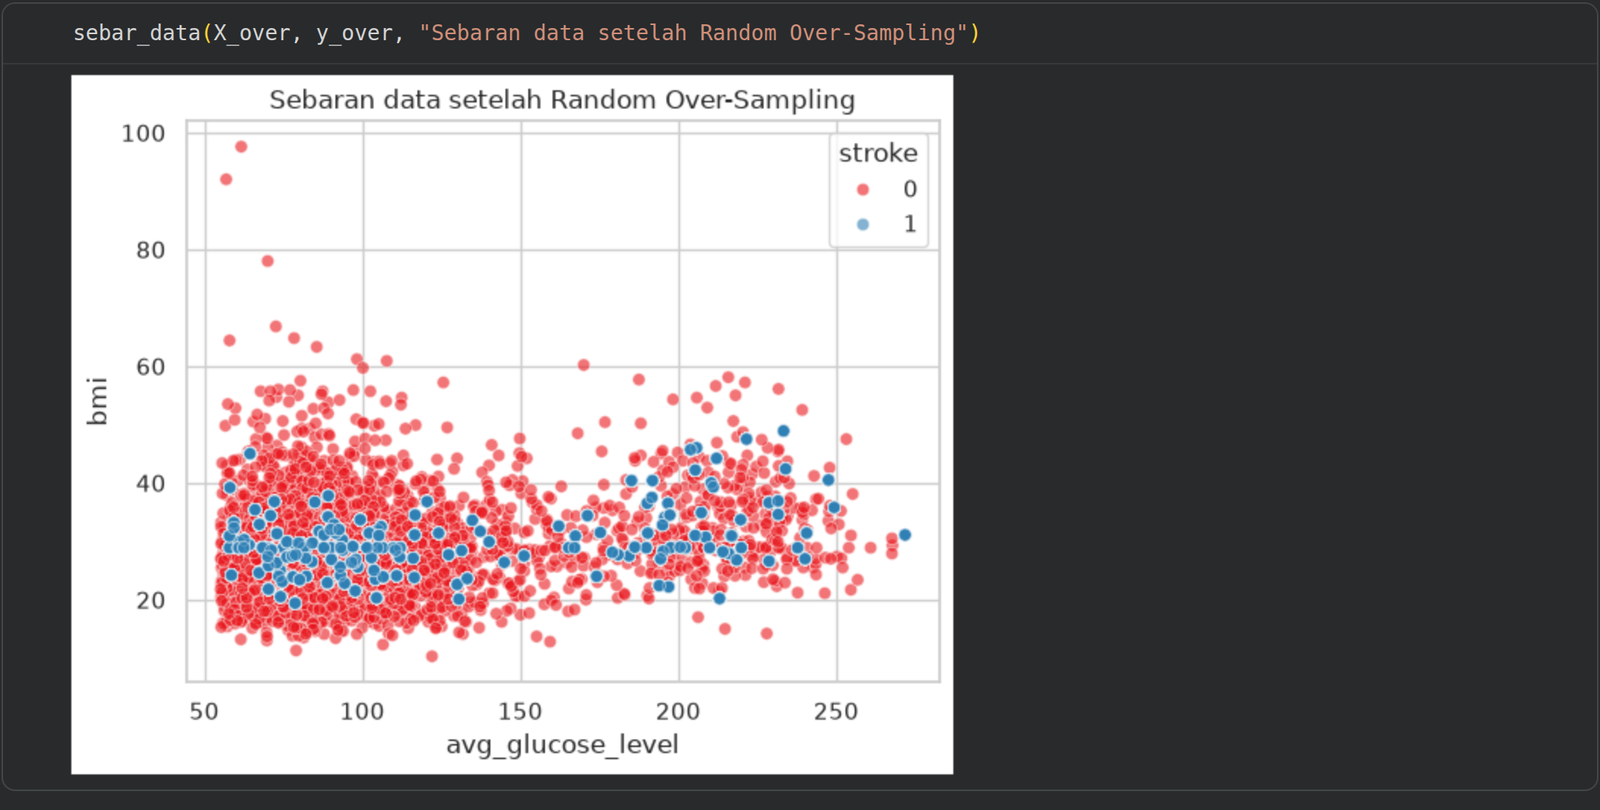
\includegraphics[width=0.68\textwidth]{images/ss-13-scatter-oversampling.png}
\caption{Sebaran data setelah \textit{Random Over-Sampling}. Titik minoritas menumpuk tepat di posisi aslinya karena hasil duplikasi.}
\label{fig:ss-scatter-ros}
\end{figure}

Pada Gambar~\ref{fig:ss-scatter-ros} terlihat titik kelas minoritas menumpuk persis di koordinat yang sama. Penumpukan ini yang membedakan duplikasi dari pembangkitan data sintetis: sebaran tidak bertambah luas, hanya kepadatannya yang berlipat.

\subsection{SMOTE}
SMOTE membangkitkan sampel sintetis di antara tetangga terdekat kelas minoritas, bukan menduplikasi sampel yang ada.

\begin{lstlisting}[style=pythonstyle,caption={Penerapan SMOTE pada set pelatihan.}]
smote = SMOTE(random_state=0)
X_smote, y_smote = smote.fit_resample(X_train, y_train)
print("Sebelum:", pd.Series(y_train).value_counts().to_dict())
print("Sesudah:", pd.Series(y_smote).value_counts().to_dict())
\end{lstlisting}

\begin{figure}[H]
\centering
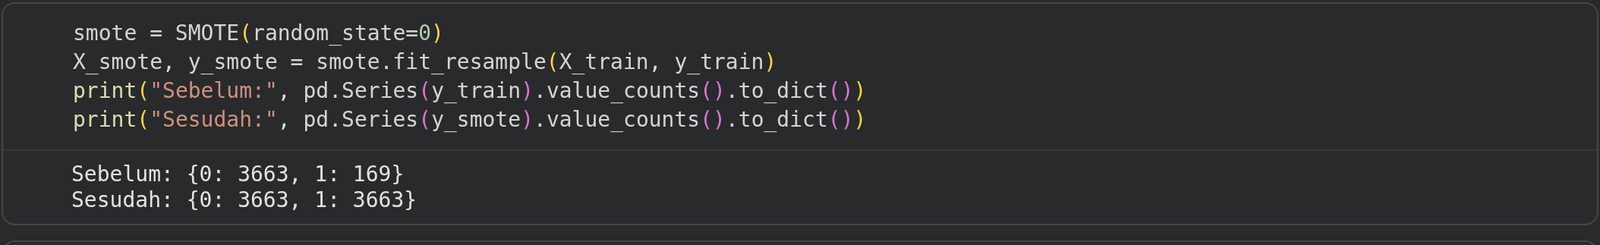
\includegraphics[width=0.7\textwidth]{images/ss-14-smote.png}
\caption{Tangkapan layar distribusi kelas sebelum dan sesudah SMOTE.}
\label{fig:ss-smote}
\end{figure}

Hasilnya setara dengan \textit{Random Over-Sampling} dari sisi jumlah, yaitu 3.663 sampel per kelas dan 7.326 baris total. Bedanya ada pada asal sampel: 3.494 sampel minoritas pada SMOTE adalah data sintetis baru, bukan salinan data lama.

\begin{figure}[H]
\centering
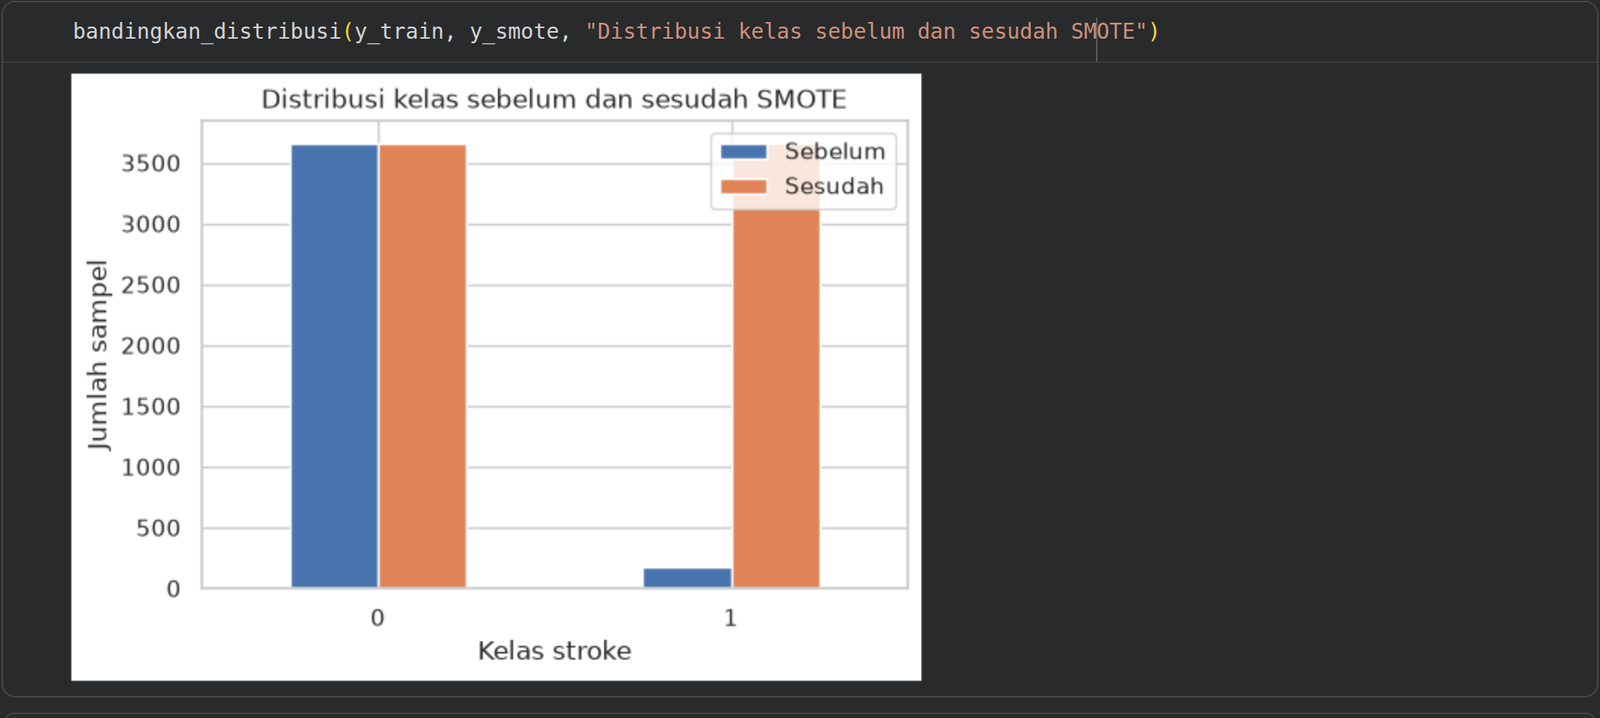
\includegraphics[width=0.68\textwidth]{images/ss-15-banding-smote.png}
\caption{Perbandingan jumlah sampel per kelas sebelum dan sesudah SMOTE.}
\label{fig:ss-banding-smote}
\end{figure}

\begin{figure}[H]
\centering
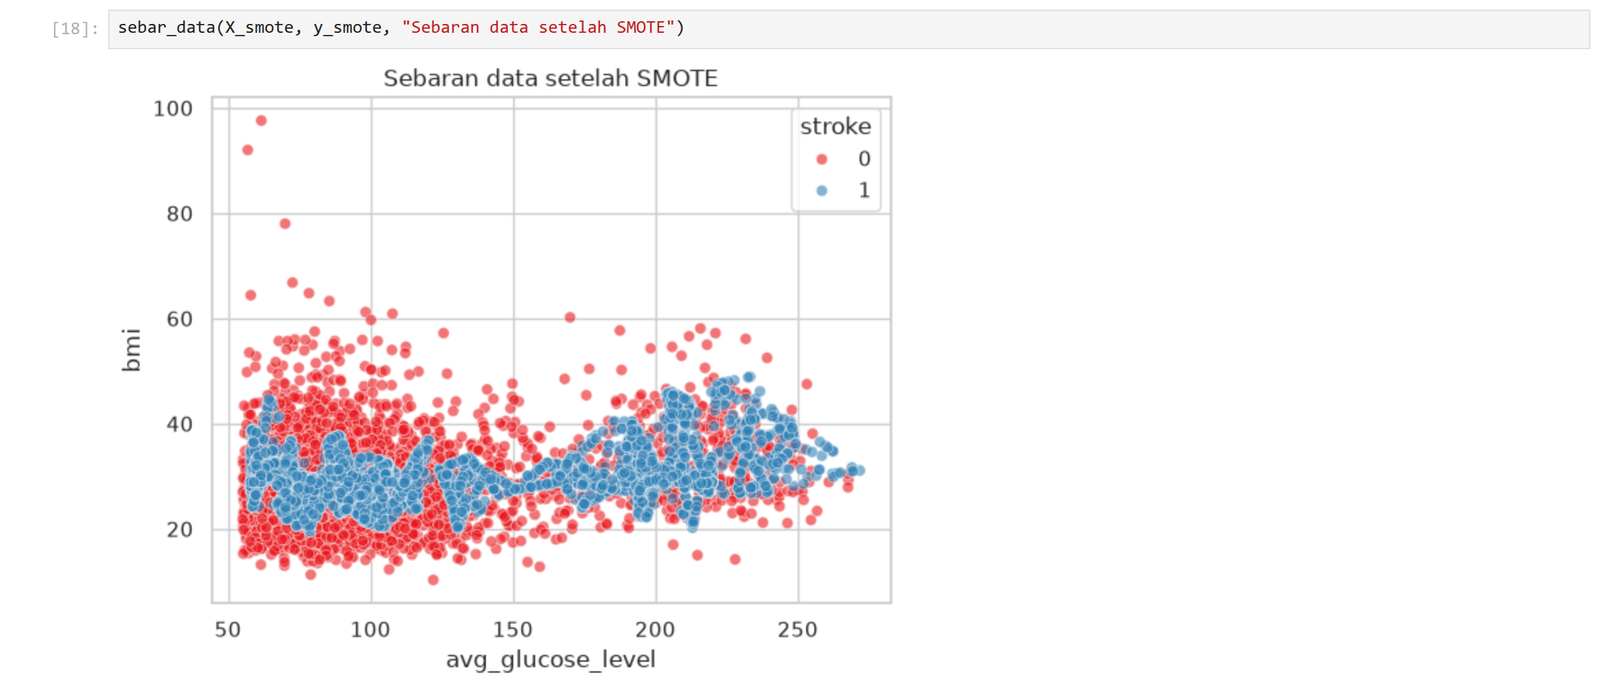
\includegraphics[width=0.68\textwidth]{images/ss-16-scatter-smote.png}
\caption{Sebaran data setelah SMOTE. Titik minoritas menyebar mengikuti garis penghubung antar-tetangga, tidak menumpuk di satu koordinat.}
\label{fig:ss-scatter-smote}
\end{figure}

Perbedaan visualnya jelas dibandingkan Gambar~\ref{fig:ss-scatter-ros}. Pada SMOTE, wilayah kelas minoritas melebar karena titik sintetis mengisi ruang di antara sampel asli. Sebaran seperti ini memberi model variasi pola yang lebih kaya dibanding duplikasi murni.

\subsection{ADASYN}
ADASYN memberi porsi pembangkitan lebih besar pada sampel minoritas yang berdekatan dengan kelas mayoritas, karena sampel seperti itu paling sulit dipisahkan.

\begin{lstlisting}[style=pythonstyle,caption={Penerapan ADASYN pada set pelatihan.}]
adasyn = ADASYN(random_state=0)
X_adasyn, y_adasyn = adasyn.fit_resample(X_train, y_train)
print("Sebelum:", pd.Series(y_train).value_counts().to_dict())
print("Sesudah:", pd.Series(y_adasyn).value_counts().to_dict())
\end{lstlisting}

\begin{figure}[H]
\centering
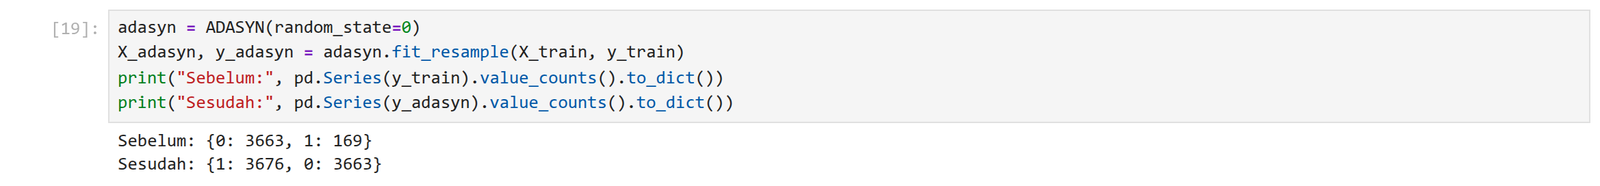
\includegraphics[width=0.7\textwidth]{images/ss-17-adasyn.png}
\caption{Tangkapan layar distribusi kelas sebelum dan sesudah ADASYN.}
\label{fig:ss-adasyn}
\end{figure}

Kelas minoritas berakhir dengan 3.676 sampel, tiga belas lebih banyak dari kelas mayoritas. Angka itu muncul karena mekanisme ADASYN membagi kuota sintetis menurut bobot kesulitan tiap sampel, sehingga totalnya bisa sedikit melewati jumlah kelas mayoritas. Total set pelatihan menjadi 7.339 baris.

\begin{figure}[H]
\centering
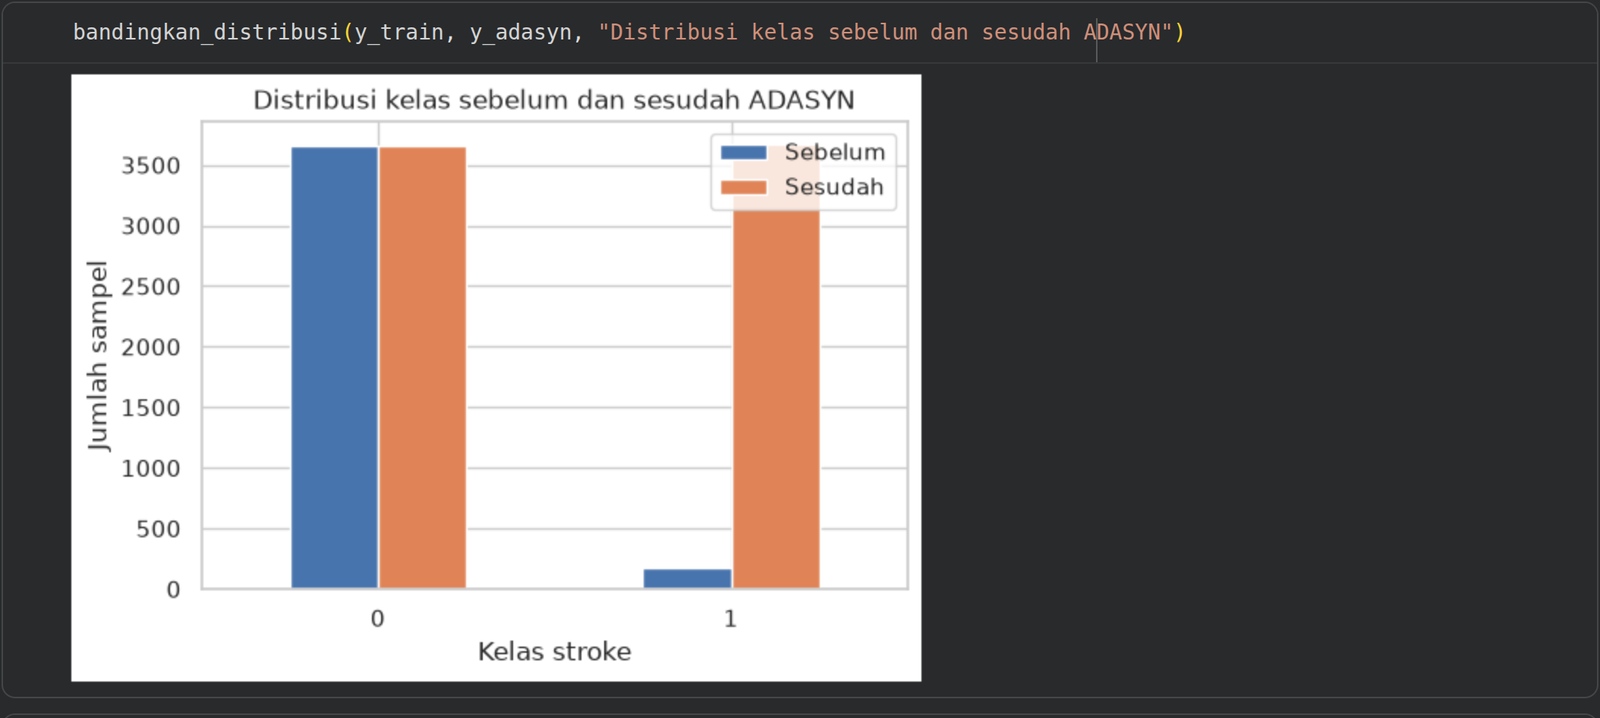
\includegraphics[width=0.68\textwidth]{images/ss-18-banding-adasyn.png}
\caption{Perbandingan jumlah sampel per kelas sebelum dan sesudah ADASYN.}
\label{fig:ss-banding-adasyn}
\end{figure}

\begin{figure}[H]
\centering
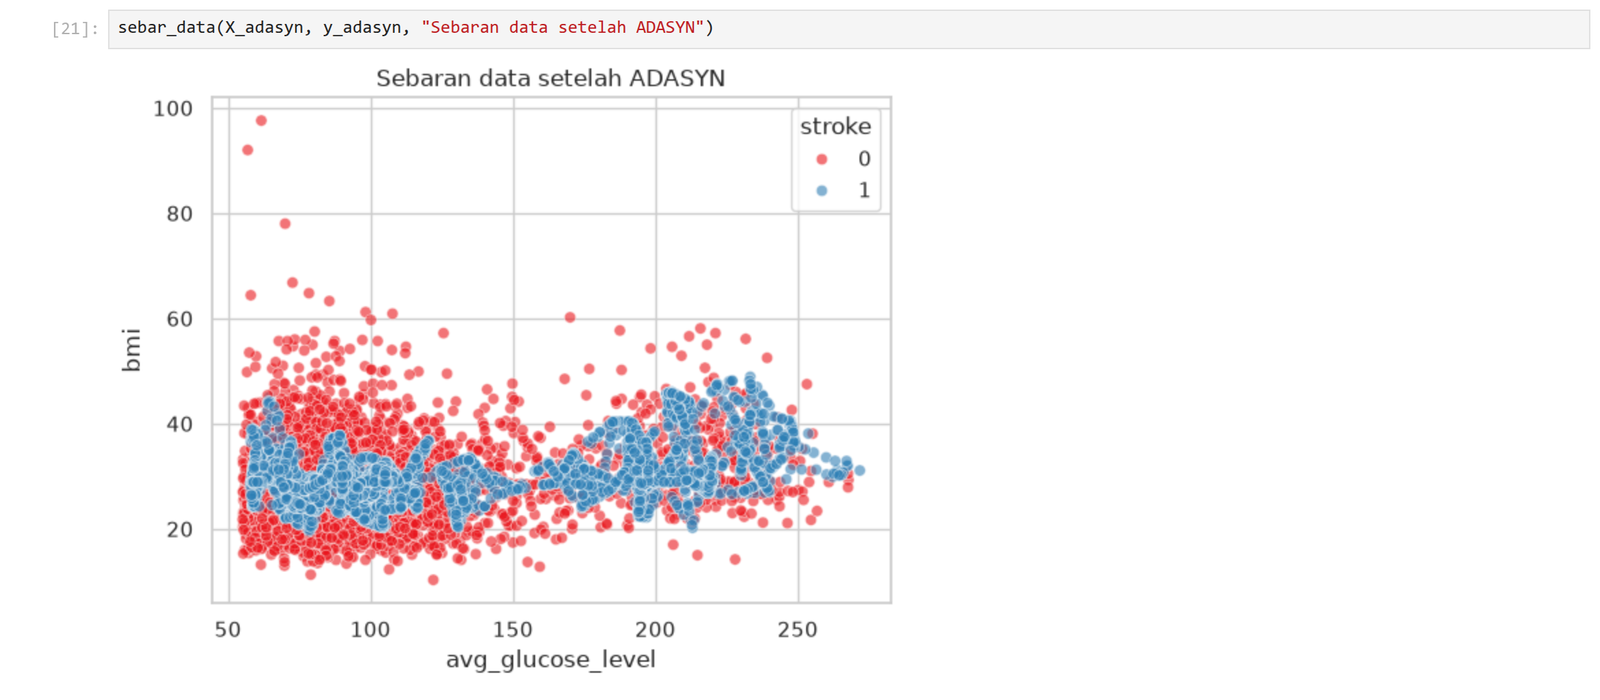
\includegraphics[width=0.68\textwidth]{images/ss-19-scatter-adasyn.png}
\caption{Sebaran data setelah ADASYN. Titik sintetis lebih terkonsentrasi di sekitar batas kedua kelas.}
\label{fig:ss-scatter-adasyn}
\end{figure}

Tabel~\ref{tab:rekap-balancing} merangkum keempat percobaan penyeimbangan pada set pelatihan yang sama.

\begin{table}[H]
\centering
\caption{Rekapitulasi hasil empat teknik penyeimbangan kelas pada set pelatihan dataset stroke.}
\label{tab:rekap-balancing}
\small
\begin{tabularx}{\linewidth}{|l|r|r|r|r|>{\raggedright\arraybackslash}X|}
\hline
\textbf{Teknik} & \textbf{Kelas 0} & \textbf{Kelas 1} & \textbf{Total} & \textbf{Sampel baru} & \textbf{Catatan} \\
\hline
Tanpa balancing & 3.663 & 169 & 3.832 & 0 & Data asli \\
\hline
\textit{Under-sampling} & 169 & 169 & 338 & 0 & 3.494 sampel mayoritas dibuang \\
\hline
\textit{Over-sampling} & 3.663 & 3.663 & 7.326 & 3.494 & Duplikasi sampel minoritas \\
\hline
SMOTE & 3.663 & 3.663 & 7.326 & 3.494 & Sampel sintetis di antara tetangga \\
\hline
ADASYN & 3.663 & 3.676 & 7.339 & 3.507 & Sintetis terpusat di batas kelas \\
\hline
\end{tabularx}
\end{table}

\subsection{Seleksi Fitur dengan Filter ANOVA}
Percobaan seleksi fitur memakai \textit{Heart Attack Analysis and Prediction Dataset} yang berisi 303 baris dan 14 kolom: 13 fitur prediktor dan satu label \texttt{output}. Dataset ini dipilih karena jumlah fiturnya cukup banyak untuk diuji, sementara labelnya masih cukup seimbang sehingga pengaruh seleksi fitur tidak tercampur dengan pengaruh penyeimbangan kelas.

\begin{lstlisting}[style=pythonstyle,caption={Membaca dataset heart.csv.}]
URL_HEART = ("https://raw.githubusercontent.com/ganjar87/"
             "data_science_practice/main/heart.csv")
jantung = pd.read_csv(URL_HEART)
print("Dimensi dataset:", jantung.shape)
print(jantung["output"].value_counts())
jantung.head()
\end{lstlisting}

\begin{figure}[H]
\centering
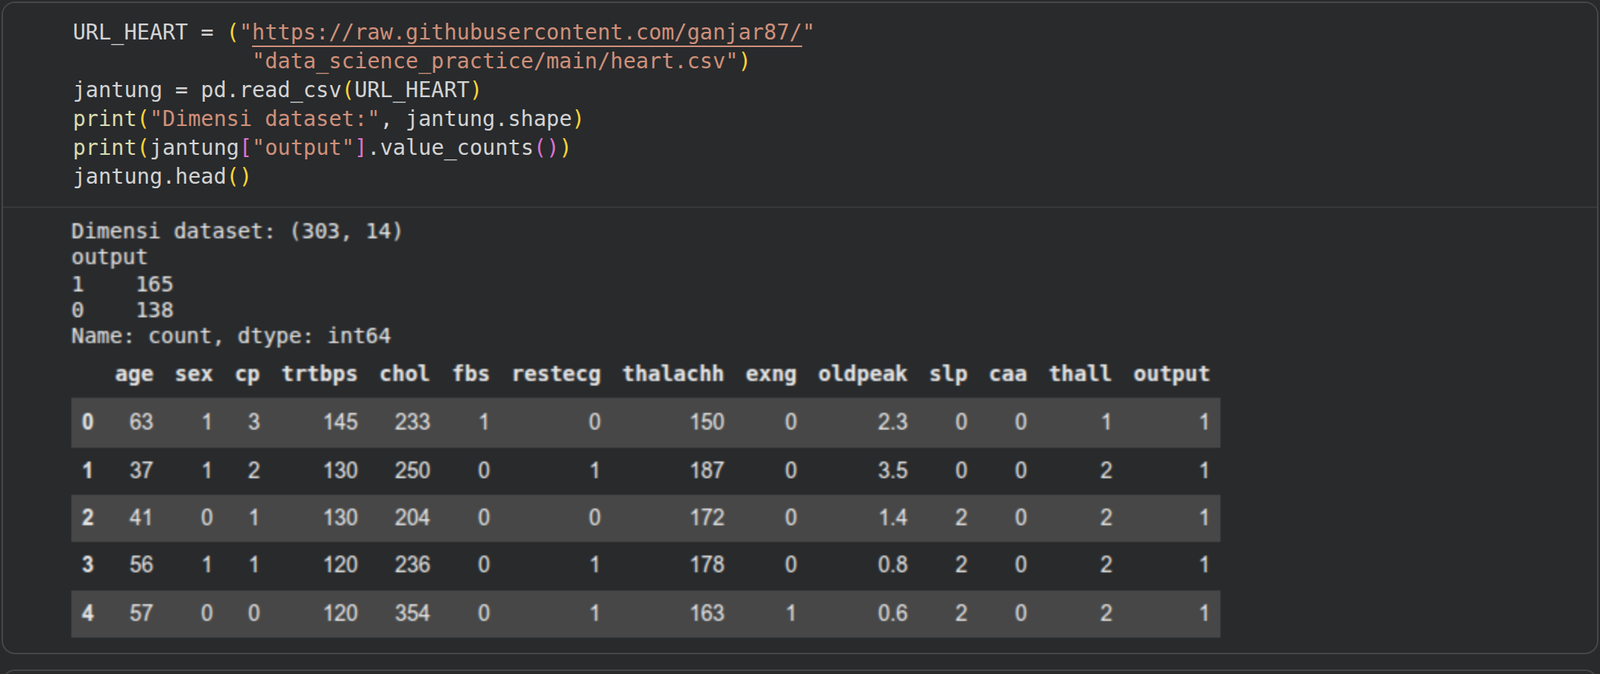
\includegraphics[width=0.9\textwidth]{images/ss-20-baca-heart.png}
\caption{Tangkapan layar pembacaan dataset heart.csv dan lima baris pertamanya.}
\label{fig:ss-heart}
\end{figure}

Label \texttt{output} terbagi menjadi 165 sampel kelas 1 dan 138 sampel kelas 0. Komposisi ini masih tergolong wajar untuk klasifikasi biner.

Uji ANOVA dijalankan dengan fungsi \texttt{f\_classif} yang menghitung nilai $F$ dan $p$ untuk setiap fitur terhadap label.

\begin{lstlisting}[style=pythonstyle,caption={Menghitung skor $F$ dan nilai $p$ setiap fitur dengan uji ANOVA.}]
X_jantung = jantung.drop(columns="output")
y_jantung = jantung["output"]

skor_f, nilai_p = f_classif(X_jantung, y_jantung)
anova = (pd.DataFrame({"F": skor_f, "p_value": nilai_p}, index=X_jantung.columns)
         .sort_values("F", ascending=False).round(4))
anova
\end{lstlisting}

\begin{figure}[H]
\centering
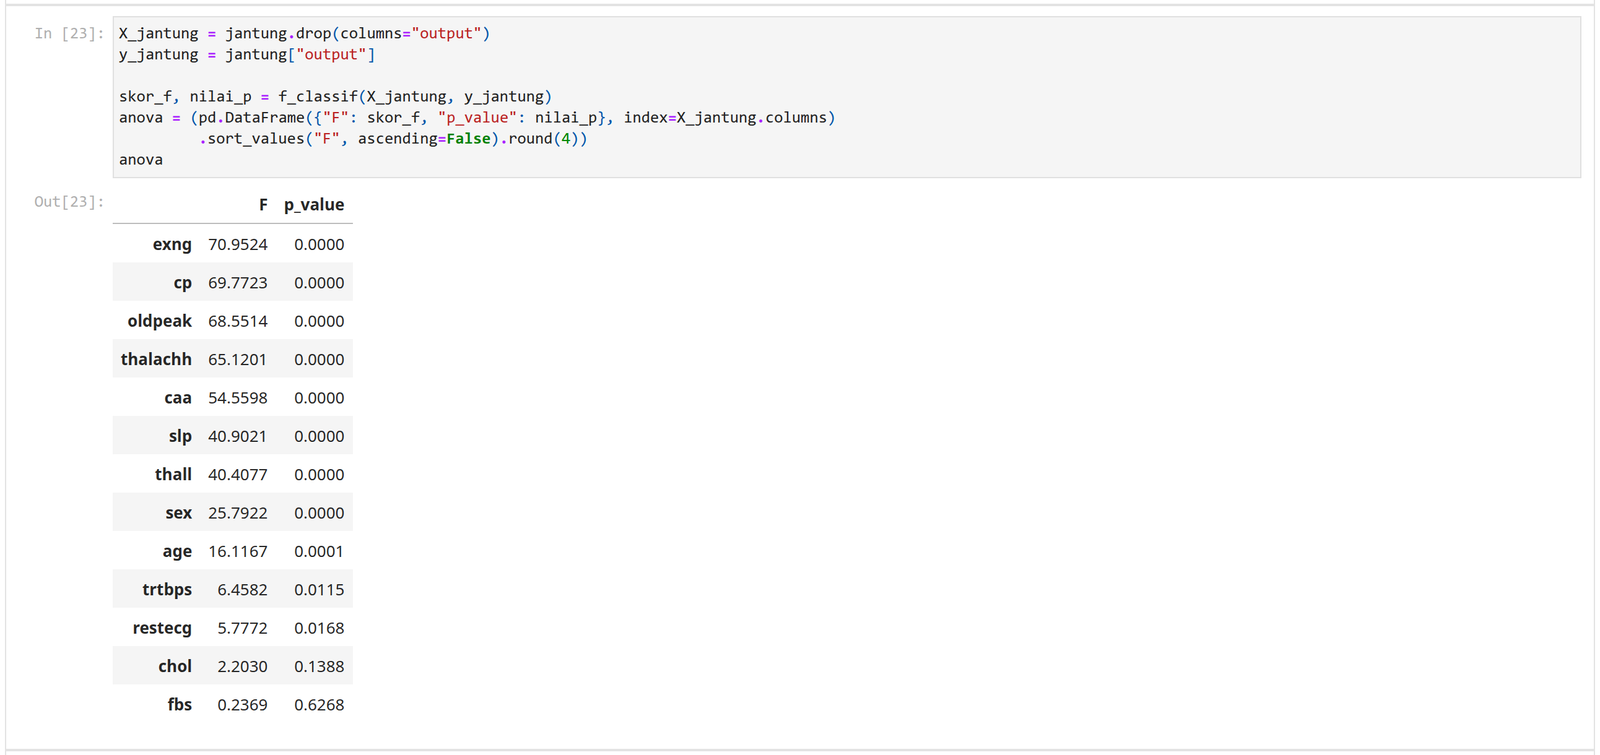
\includegraphics[width=0.6\textwidth]{images/ss-21-anova-ranking.png}
\caption{Tangkapan layar peringkat fitur menurut skor $F$ hasil uji ANOVA.}
\label{fig:ss-anova}
\end{figure}

Hasil lengkapnya disusun pada Tabel~\ref{tab:anova}.

\begin{table}[H]
\centering
\caption{Peringkat fitur dataset heart berdasarkan skor $F$ uji ANOVA.}
\label{tab:anova}
\small
\begin{tabular}{|l|r|r|l|r|r|}
\hline
\textbf{Fitur} & \textbf{$F$} & \textbf{$p$} & \textbf{Fitur} & \textbf{$F$} & \textbf{$p$} \\
\hline
\texttt{exng} & 70,9524 & 0,0000 & \texttt{sex} & 25,7922 & 0,0000 \\
\hline
\texttt{cp} & 69,7723 & 0,0000 & \texttt{age} & 16,1167 & 0,0001 \\
\hline
\texttt{oldpeak} & 68,5514 & 0,0000 & \texttt{trtbps} & 6,4582 & 0,0115 \\
\hline
\texttt{thalachh} & 65,1201 & 0,0000 & \texttt{restecg} & 5,7772 & 0,0168 \\
\hline
\texttt{caa} & 54,5598 & 0,0000 & \texttt{chol} & 2,2030 & 0,1388 \\
\hline
\texttt{slp} & 40,9021 & 0,0000 & \texttt{fbs} & 0,2369 & 0,6268 \\
\hline
\texttt{thall} & 40,4077 & 0,0000 & & & \\
\hline
\end{tabular}
\end{table}

Delapan fitur teratas dipilih sebagai subset hasil \textit{filter method}. Batas delapan diambil untuk menyisakan sekitar separuh fitur, sehingga pengurangan dimensi cukup terasa tanpa membuang fitur yang masih informatif.

\begin{lstlisting}[style=pythonstyle,caption={Mengambil delapan fitur dengan skor $F$ tertinggi.}]
fitur_anova = anova.index[:8].tolist()
print("Fitur terpilih (ANOVA):", fitur_anova)
\end{lstlisting}

\begin{figure}[H]
\centering
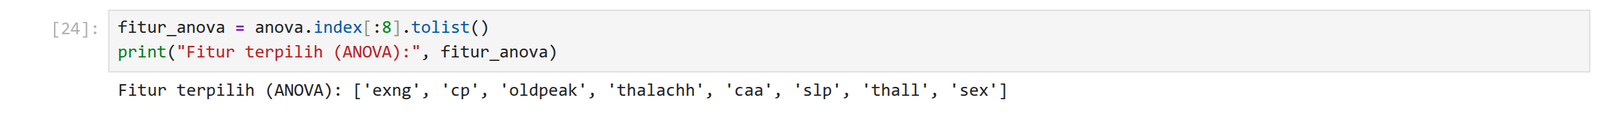
\includegraphics[width=0.75\textwidth]{images/ss-22-fitur-anova.png}
\caption{Tangkapan layar delapan fitur terpilih hasil uji ANOVA.}
\label{fig:ss-fitur-anova}
\end{figure}

Tiga fitur terbawah, yaitu \texttt{restecg}, \texttt{chol}, dan \texttt{fbs}, memiliki $p > 0{,}01$ sehingga perbedaan rata-ratanya antar-kelas tidak cukup meyakinkan. Ketiganya otomatis tersisih oleh peringkat $F$ dan tidak masuk subset.

\subsection{Seleksi Fitur dengan Wrapper RFE}
\textit{Recursive Feature Elimination} memakai pohon keputusan sebagai penilai, membuang fitur dengan bobot terkecil pada setiap iterasi, lalu berhenti saat jumlah fitur mencapai target lima.

\begin{lstlisting}[style=pythonstyle,caption={Seleksi lima fitur dengan RFE.}]
rfe = RFE(estimator=DecisionTreeClassifier(random_state=42), n_features_to_select=5)
rfe.fit(X_jantung, y_jantung)
fitur_rfe = X_jantung.columns[rfe.support_].tolist()
print("Fitur terpilih (RFE):", fitur_rfe)
\end{lstlisting}

\begin{figure}[H]
\centering
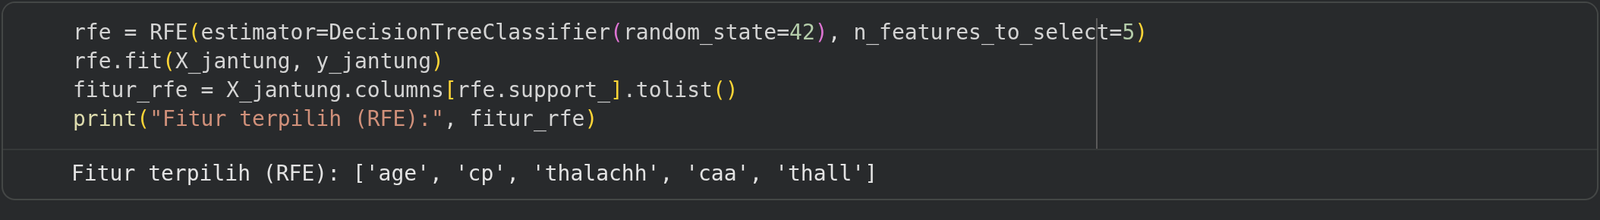
\includegraphics[width=0.75\textwidth]{images/ss-23-fitur-rfe.png}
\caption{Tangkapan layar lima fitur terpilih hasil RFE.}
\label{fig:ss-fitur-rfe}
\end{figure}

Lima fitur yang bertahan adalah \texttt{age}, \texttt{cp}, \texttt{thalachh}, \texttt{caa}, dan \texttt{thall}. Susunan ini berbeda dari contoh pada materi kuliah yang menyisakan \texttt{sex}, \texttt{exng}, \texttt{slp}, \texttt{caa}, dan \texttt{thall}. Perbedaan itu wajar karena urutan eliminasi bergantung pada pohon yang terbentuk di setiap iterasi, dan pohon itu dipengaruhi \textit{random\_state} serta versi pustaka. Yang penting, kedua hasil sama-sama menyisakan lima fitur dengan \texttt{caa} dan \texttt{thall} sebagai irisan.

\subsection{Seleksi Fitur dengan Embedded ExtraTree}
\textit{ExtraTreesClassifier} menghitung \textit{feature importance} selama pelatihan, sehingga seleksi berjalan tanpa proses berulang yang terpisah.

\begin{lstlisting}[style=pythonstyle,caption={Menghitung \textit{feature importance} dengan ExtraTree.}]
extra = ExtraTreesClassifier(random_state=42)
extra.fit(X_jantung, y_jantung)
kepentingan = (pd.Series(extra.feature_importances_, index=X_jantung.columns)
               .sort_values(ascending=False).round(4))
print(kepentingan)

fitur_extra = kepentingan.index[:6].tolist()
print("Fitur terpilih (ExtraTree):", fitur_extra)
\end{lstlisting}

\begin{figure}[H]
\centering
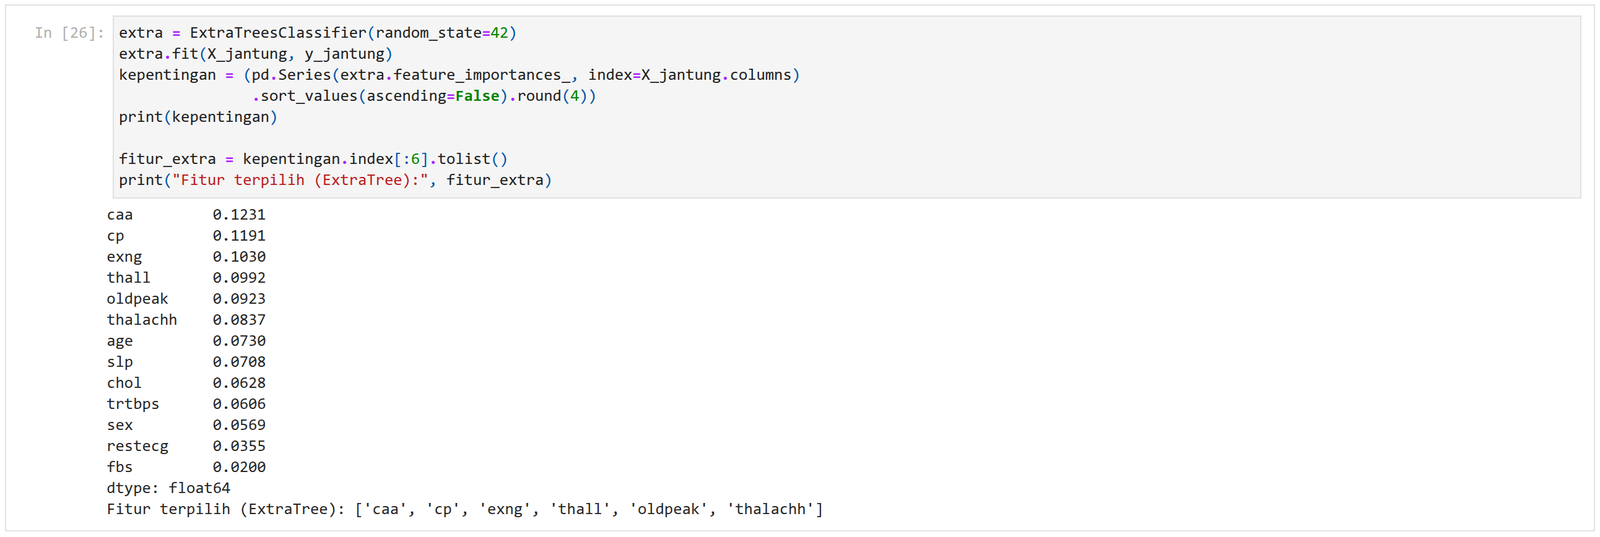
\includegraphics[width=0.7\textwidth]{images/ss-24-fitur-extratree.png}
\caption{Tangkapan layar peringkat \textit{feature importance} dan enam fitur terpilih hasil ExtraTree.}
\label{fig:ss-fitur-extra}
\end{figure}

Enam fitur teratas adalah \texttt{caa} (0,1231), \texttt{cp} (0,1191), \texttt{exng} (0,1030), \texttt{thall} (0,0992), \texttt{oldpeak} (0,0923), dan \texttt{thalachh} (0,0837). Himpunan ini identik dengan delapan fitur hasil ANOVA tanpa \texttt{slp} dan \texttt{sex}. Kesamaan tersebut masuk akal karena keduanya menilai kemampuan fitur memisahkan kelas, hanya metriknya yang berbeda.

\subsection{Komparasi Metode Seleksi Fitur dan Pemeriksaan Overfitting}
Ketiga subset fitur diuji dengan pengklasifikasi yang sama pada pembagian data yang sama, yaitu \texttt{DecisionTreeClassifier} dengan \texttt{random\_state=42} dan rasio 80:20.

\begin{lstlisting}[style=pythonstyle,caption={Membandingkan akurasi latih dan uji pada empat skenario fitur.}]
def akurasi_pohon(kolom):
    X_latih, X_uji, y_latih, y_uji = train_test_split(
        X_jantung[kolom], y_jantung, test_size=0.2, random_state=42)
    model = DecisionTreeClassifier(random_state=42).fit(X_latih, y_latih)
    return (round(accuracy_score(y_latih, model.predict(X_latih)), 3),
            round(accuracy_score(y_uji, model.predict(X_uji)), 3))


skenario = {
    "Tanpa seleksi": X_jantung.columns.tolist(),
    "Filter ANOVA": fitur_anova,
    "Wrapper RFE": fitur_rfe,
    "Embedded ExtraTree": fitur_extra,
}

hasil_seleksi = pd.DataFrame(
    [(nama, len(kolom), *akurasi_pohon(kolom)) for nama, kolom in skenario.items()],
    columns=["Metode", "Jumlah fitur", "Akurasi latih", "Akurasi uji"])
hasil_seleksi
\end{lstlisting}

\begin{figure}[H]
\centering
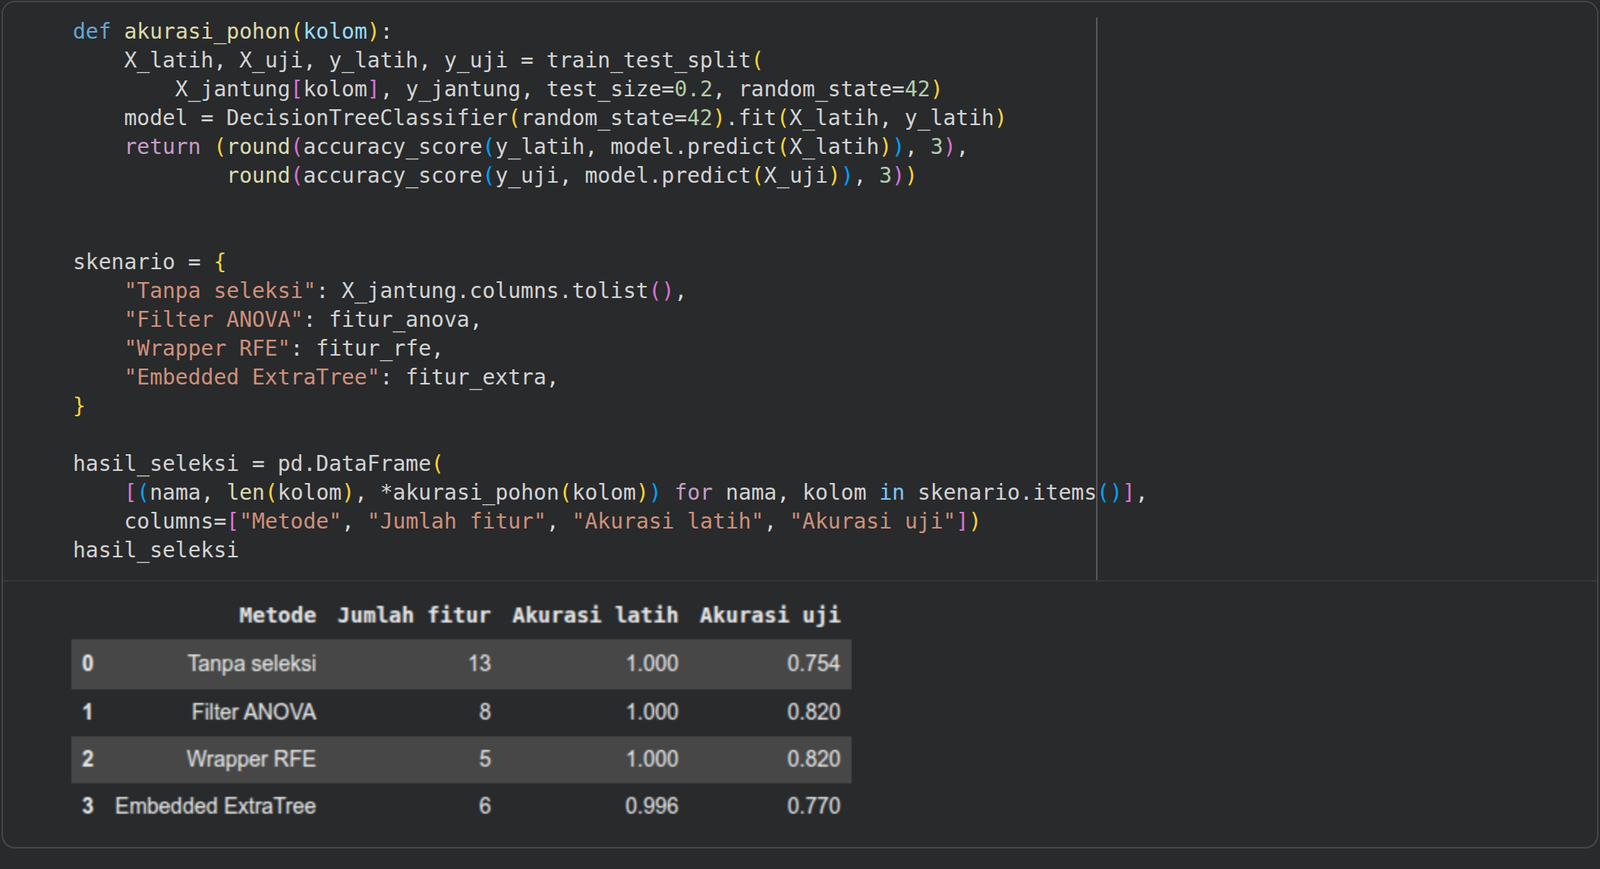
\includegraphics[width=0.9\textwidth]{images/ss-25-komparasi-seleksi.png}
\caption{Tangkapan layar tabel perbandingan akurasi empat skenario seleksi fitur.}
\label{fig:ss-komparasi}
\end{figure}

Hasilnya dirangkum pada Tabel~\ref{tab:seleksi}.

\begin{table}[H]
\centering
\caption{Perbandingan akurasi \textit{Decision Tree} pada empat skenario seleksi fitur dataset heart.}
\label{tab:seleksi}
\small
\begin{tabularx}{\linewidth}{|l|r|l|>{\raggedright\arraybackslash}X|}
\hline
\textbf{Skenario} & \textbf{Jumlah fitur} & \textbf{Akurasi uji} & \textbf{Fitur yang dipakai} \\
\hline
Tanpa seleksi & 13 & 0,754 & Seluruh fitur \\
\hline
\textit{Filter} ANOVA & 8 & 0,820 & \texttt{exng}, \texttt{cp}, \texttt{oldpeak}, \texttt{thalachh}, \texttt{caa}, \texttt{slp}, \texttt{thall}, \texttt{sex} \\
\hline
\textit{Wrapper} RFE & 5 & 0,820 & \texttt{age}, \texttt{cp}, \texttt{thalachh}, \texttt{caa}, \texttt{thall} \\
\hline
\textit{Embedded} ExtraTree & 6 & 0,770 & \texttt{caa}, \texttt{cp}, \texttt{exng}, \texttt{thall}, \texttt{oldpeak}, \texttt{thalachh} \\
\hline
\end{tabularx}
\end{table}

Pemangkasan fitur menaikkan akurasi uji dari 0,754 menjadi 0,820, atau 6,6 poin persen. RFE memberi hasil terbaik dari sisi efisiensi karena hanya memakai lima fitur untuk akurasi yang sama dengan ANOVA yang memakai delapan fitur. ExtraTree sedikit tertinggal pada percobaan ini meski jumlah fiturnya hanya enam.

Satu hal yang mencolok pada tabel tersebut: akurasi latih menyentuh 1,000 pada tiga skenario. Pohon keputusan tanpa batas kedalaman memang sanggup menghafal seluruh data latih. Untuk memastikan jarak itu benar-benar gejala \textit{overfitting}, saya membandingkan pohon penuh dengan pohon yang kedalamannya dibatasi.

\begin{lstlisting}[style=pythonstyle,caption={Membandingkan pohon penuh dengan pohon yang dipangkas.}]
X_latih, X_uji, y_latih, y_uji = train_test_split(
    X_jantung[fitur_extra], y_jantung, test_size=0.2, random_state=42)

pohon_penuh = DecisionTreeClassifier(random_state=42).fit(X_latih, y_latih)
pohon_pangkas = DecisionTreeClassifier(max_depth=3, random_state=42).fit(X_latih, y_latih)

pd.DataFrame({
    "Model": ["Pohon penuh", "Pohon dipangkas (max_depth=3)"],
    "Kedalaman": [pohon_penuh.get_depth(), pohon_pangkas.get_depth()],
    "Jumlah daun": [pohon_penuh.get_n_leaves(), pohon_pangkas.get_n_leaves()],
    "Akurasi latih": [round(accuracy_score(y_latih, pohon_penuh.predict(X_latih)), 3),
                      round(accuracy_score(y_latih, pohon_pangkas.predict(X_latih)), 3)],
    "Akurasi uji": [round(accuracy_score(y_uji, pohon_penuh.predict(X_uji)), 3),
                    round(accuracy_score(y_uji, pohon_pangkas.predict(X_uji)), 3)],
})
\end{lstlisting}

\begin{figure}[H]
\centering
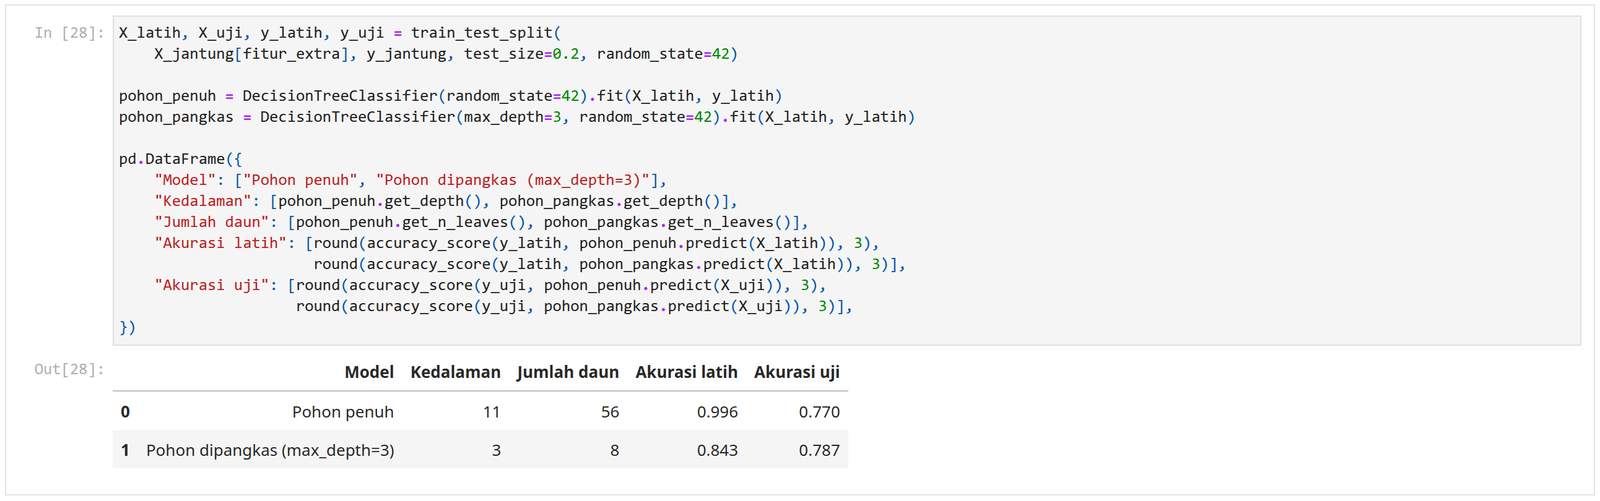
\includegraphics[width=0.9\textwidth]{images/ss-26-overfitting-pangkas.png}
\caption{Tangkapan layar perbandingan kedalaman, jumlah daun, dan akurasi pohon penuh dengan pohon yang dipangkas.}
\label{fig:ss-overfitting}
\end{figure}

\begin{table}[H]
\centering
\caption{Pengaruh pemangkasan kedalaman terhadap selisih akurasi latih dan uji.}
\label{tab:overfitting}
\small
\setlength{\tabcolsep}{4.5pt}
\begin{tabular}{|l|r|r|r|r|}
\hline
\textbf{Model} & \textbf{Kedalaman} & \textbf{Jumlah daun} & \textbf{Akurasi latih} & \textbf{Akurasi uji} \\
\hline
Pohon penuh & 11 & 56 & 0,996 & 0,770 \\
\hline
Pohon dipangkas (\texttt{max\_depth=3}) & 3 & 8 & 0,843 & 0,787 \\
\hline
\end{tabular}
\end{table}

Pohon penuh tumbuh sampai kedalaman 11 dengan 56 daun. Akurasi latihnya 0,996, sementara akurasi ujinya hanya 0,770. Jarak 0,226 di antara keduanya adalah tanda pohon menghafal data latih, termasuk derau yang tidak akan muncul lagi di data baru. Setelah kedalaman dibatasi menjadi 3, jumlah daun turun ke 8, akurasi latih turun ke 0,843, tetapi akurasi uji justru naik ke 0,787. Jaraknya menyempit dari 0,226 menjadi 0,056. Model yang lebih sederhana ternyata lebih mampu menggeneralisasi.

\section{Tugas dan Analisis Praktikum}

\subsection{Tugas 1: Eksplorasi Dataset Stroke}
Tugas pertama meminta penjelasan tujuan dataset dan arti setiap fitur. \textit{Stroke Prediction Dataset} dipakai untuk membangun model klasifikasi yang memperkirakan apakah seorang pasien berpotensi mengalami stroke berdasarkan data klinis dan demografis. Dalam konteks penambangan data, dataset ini menjadi contoh kasus klasifikasi medis dengan kelas tidak seimbang yang ekstrem, yaitu 4,87\% positif. Pola seperti ini menuntut perlakuan khusus pada tahap persiapan data, dan sekaligus menjadi alasan mengapa akurasi bukan metrik tunggal yang layak dipakai.

\begin{lstlisting}[style=pythonstyle,caption={Merangkum tipe data, jumlah nilai unik, nilai kosong, dan contoh nilai tiap fitur.}]
pd.DataFrame({
    "Tipe data": stroke.dtypes.astype(str),
    "Nilai unik": stroke.nunique(),
    "Nilai hilang": stroke.isnull().sum(),
    "Contoh": [stroke[k].dropna().iloc[0] for k in stroke.columns],
})
\end{lstlisting}

\begin{figure}[H]
\centering
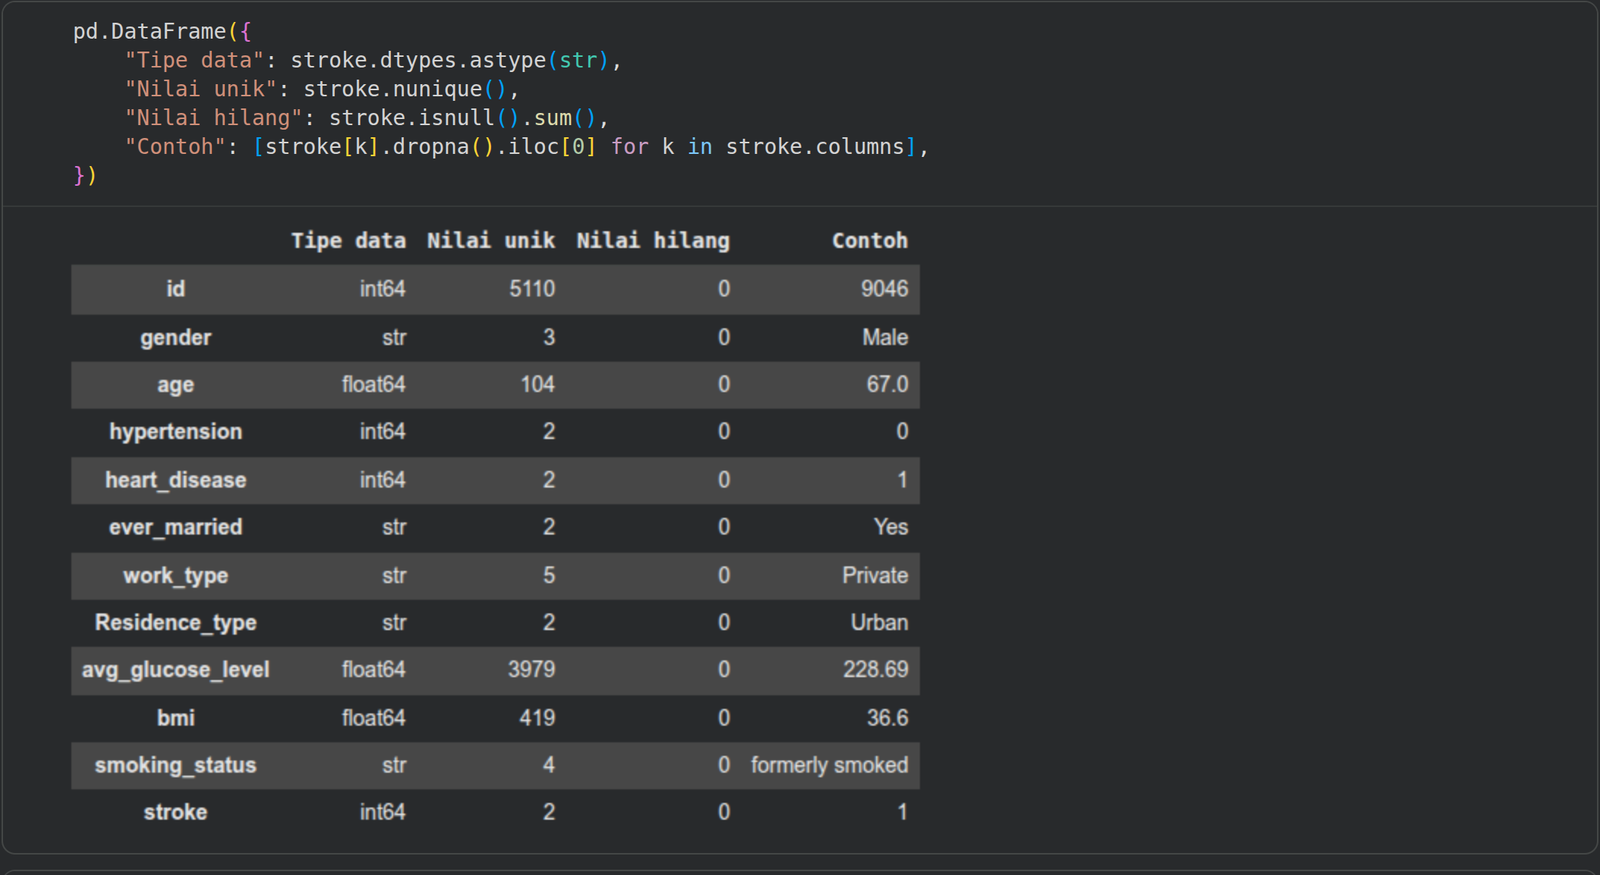
\includegraphics[width=0.95\textwidth]{images/ss-27-tugas1-ringkasan-fitur.png}
\caption{Tangkapan layar ringkasan tipe data, jumlah nilai unik, nilai kosong, dan contoh nilai setiap kolom.}
\label{fig:ss-ringkasan-fitur}
\end{figure}

\begin{figure}[H]
\centering
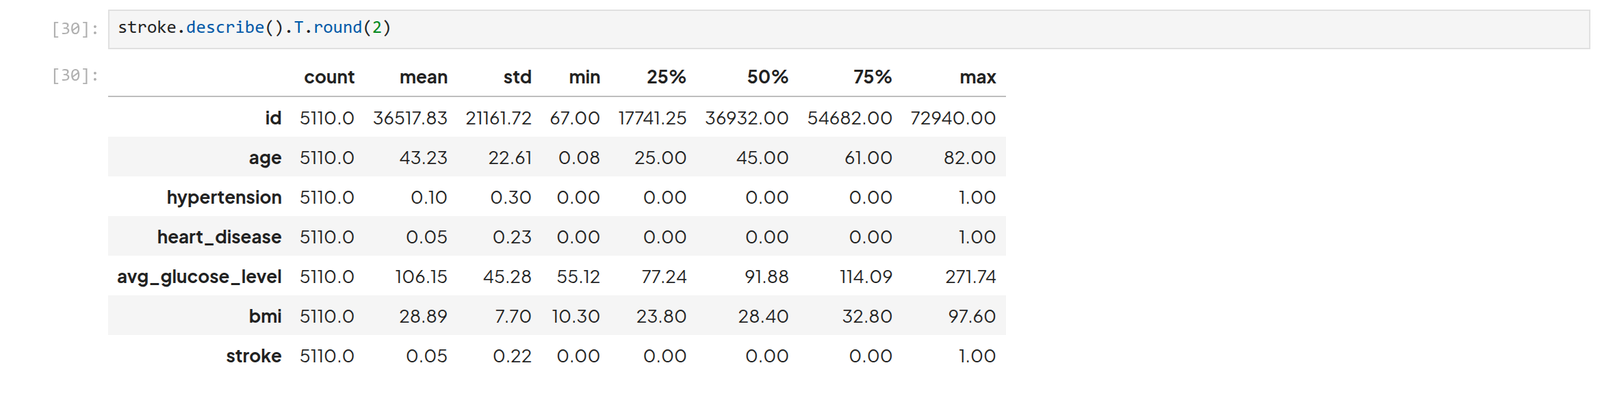
\includegraphics[width=0.85\textwidth]{images/ss-28-tugas1-statistik.png}
\caption{Tangkapan layar statistik deskriptif fitur numerik dataset stroke.}
\label{fig:ss-statistik}
\end{figure}

Penjelasan setiap fitur disusun pada Tabel~\ref{tab:fitur-stroke}.

\begin{table}[H]
\centering
\caption{Arti setiap fitur pada \textit{Stroke Prediction Dataset}.}
\label{tab:fitur-stroke}
\small
\begin{tabularx}{\linewidth}{|l|>{\raggedright\arraybackslash}p{2.6cm}|>{\raggedright\arraybackslash}X|}
\hline
\textbf{Fitur} & \textbf{Tipe} & \textbf{Arti dan rentang nilai} \\
\hline
\texttt{id} & Bilangan bulat & Nomor unik pasien, 5.110 nilai berbeda. Tidak dipakai sebagai fitur karena tidak punya makna klinis. \\
\hline
\texttt{gender} & Kategorikal & Jenis kelamin pasien: \textit{Male}, \textit{Female}, \textit{Other}. \\
\hline
\texttt{age} & Pecahan & Usia pasien dalam tahun, rentang 0,08 sampai 82 dengan rata-rata 43,23. \\
\hline
\texttt{hypertension} & Biner & Riwayat hipertensi: 0 tidak, 1 ya. Rata-rata 0,10 berarti sekitar 10\% pasien hipertensi. \\
\hline
\texttt{heart\_disease} & Biner & Riwayat penyakit jantung: 0 tidak, 1 ya. Rata-rata 0,05. \\
\hline
\texttt{ever\_married} & Kategorikal & Status pernah menikah: \textit{Yes} atau \textit{No}. \\
\hline
\texttt{work\_type} & Kategorikal & Jenis pekerjaan: \textit{Private}, \textit{Self-employed}, \textit{Govt\_job}, \textit{children}, \textit{Never\_worked}. \\
\hline
\texttt{Residence\_type} & Kategorikal & Tipe tempat tinggal: \textit{Urban} atau \textit{Rural}. \\
\hline
\texttt{avg\_glucose\_level} & Pecahan & Rata-rata kadar glukosa darah dalam mg/dL, rentang 55,12 sampai 271,74 dengan rata-rata 106,15. \\
\hline
\texttt{bmi} & Pecahan & Indeks massa tubuh dalam kg/m$^2$, rentang 10,30 sampai 97,60 dengan rata-rata 28,89. Memiliki 201 nilai kosong. \\
\hline
\texttt{smoking\_status} & Kategorikal & Status merokok: \textit{formerly smoked}, \textit{never smoked}, \textit{smokes}, \textit{Unknown}. \\
\hline
\texttt{stroke} & Biner & Label target: 1 pasien mengalami stroke, 0 tidak. Hanya 4,87\% bernilai 1. \\
\hline
\end{tabularx}
\end{table}

Dua fitur perlu perhatian khusus. \texttt{bmi} memiliki 201 nilai kosong sehingga wajib diimputasi sebelum dipakai. \texttt{age} memiliki nilai minimum 0,08 tahun, yang secara medis tidak lazim untuk data pasien stroke dan bisa jadi hasil pencatatan dalam satuan berbeda. Saya membiarkan nilai tersebut apa adanya karena modul tidak menginstruksikan pembersihan lebih lanjut, tetapi ketidakwajaran ini perlu dicatat sebagai keterbatasan dataset.

\subsection{Tugas 2: Komparasi Balancing pada Dataset Kedua}
Tugas kedua meminta perbandingan performa model sebelum dan sesudah penyeimbangan pada dataset lain. Saya memilih \textit{Wine Quality (red)} dari UCI karena labelnya bisa dibentuk menjadi klasifikasi biner yang timpang tanpa rekayasa berlebihan.

Label asli dataset ini berupa skor kualitas ordinal 3 sampai 8 dengan sebaran yang tidak merata: skor 5 dan 6 mendominasi, sedangkan skor 7 hanya 199 baris dan skor 8 hanya 18 baris. Saya mengubah label tersebut menjadi dua kelas, yaitu kualitas premium untuk skor 7 ke atas dan kualitas standar untuk skor di bawah 7. Hasilnya kelas minoritas berisi 217 baris (13,57\%) dan kelas mayoritas 1.382 baris (86,43\%), dengan rasio 6,37 banding 1.

\begin{lstlisting}[style=pythonstyle,caption={Membaca dataset Wine Quality dan membentuk label biner premium.}]
URL_WINE = "https://raw.githubusercontent.com/plotly/datasets/master/winequality-red.csv"
anggur = pd.read_csv(URL_WINE)
anggur["premium"] = (anggur["quality"] >= 7).astype(int)
anggur = anggur.drop(columns="quality")

print("Dimensi dataset:", anggur.shape)
print(anggur["premium"].value_counts())
print("Rasio ketidakseimbangan:", round(1382 / 217, 2), ": 1")
\end{lstlisting}

\begin{figure}[H]
\centering
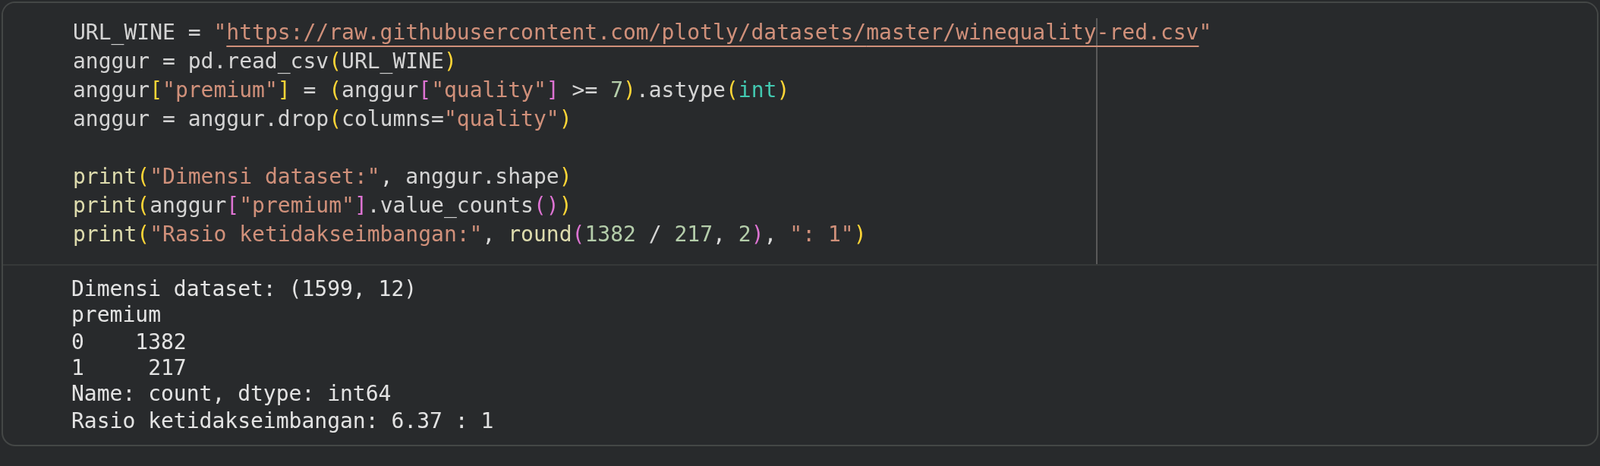
\includegraphics[width=0.85\textwidth]{images/ss-29-tugas2-wine.png}
\caption{Tangkapan layar dimensi, distribusi kelas, dan rasio ketidakseimbangan dataset Wine Quality.}
\label{fig:ss-wine}
\end{figure}

Data dibagi 75:25 dengan \texttt{stratify} agar proporsi kelas pada kedua bagian tetap sama. Pemakaian \texttt{stratify} di sini berbeda dari percobaan stroke yang mengikuti modul, karena pada dataset ini jumlah kelas minoritas cukup besar sehingga stratifikasi tidak mengubah struktur data secara berarti.

\begin{lstlisting}[style=pythonstyle,caption={Membagi data dengan stratifikasi kelas.}]
X_anggur = anggur.drop(columns="premium")
y_anggur = anggur["premium"]
X_latih_a, X_uji_a, y_latih_a, y_uji_a = train_test_split(
    X_anggur, y_anggur, test_size=0.25, random_state=42, stratify=y_anggur)

print("Latih:", pd.Series(y_latih_a).value_counts().to_dict())
print("Uji:", pd.Series(y_uji_a).value_counts().to_dict())
\end{lstlisting}

\begin{figure}[H]
\centering
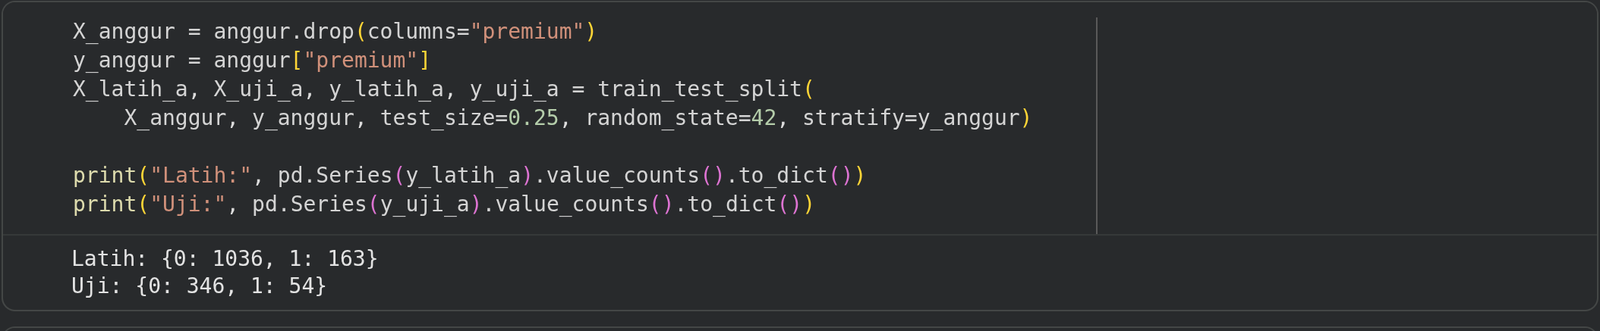
\includegraphics[width=0.8\textwidth]{images/ss-30-tugas2-split.png}
\caption{Tangkapan layar distribusi kelas pada set pelatihan dan pengujian setelah stratifikasi.}
\label{fig:ss-wine-split}
\end{figure}

Set pelatihan berisi 1.199 baris (1.036 kelas mayoritas dan 163 kelas minoritas), sedangkan set pengujian berisi 400 baris (346 dan 54). Dua pengklasifikasi dipakai, yaitu \textit{Decision Tree} dan \textit{Random Forest}, agar pola perubahannya terlihat konsisten dan tidak bergantung pada satu model.

\begin{lstlisting}[style=pythonstyle,caption={Menguji dua pengklasifikasi pada tiga kondisi penyeimbangan.}]
def evaluasi(model, X_latih, y_latih, X_uji, y_uji, label):
    model.fit(X_latih, y_latih)
    prediksi = model.predict(X_uji)
    return {
        "Model": label,
        "Accuracy": round(accuracy_score(y_uji, prediksi), 4),
        "Precision": round(precision_score(y_uji, prediksi), 4),
        "Recall": round(recall_score(y_uji, prediksi), 4),
        "F1-Score": round(f1_score(y_uji, prediksi), 4),
    }


baris = []
for nama_model, pembuat in [("Decision Tree", DecisionTreeClassifier),
                            ("Random Forest", RandomForestClassifier)]:
    baris.append(evaluasi(pembuat(random_state=42), X_latih_a, y_latih_a,
                          X_uji_a, y_uji_a, f"{nama_model} tanpa balancing"))
    for nama_sampler, sampler in [("SMOTE", SMOTE(random_state=42)),
                                  ("ADASYN", ADASYN(random_state=42))]:
        X_res, y_res = sampler.fit_resample(X_latih_a, y_latih_a)
        baris.append(evaluasi(pembuat(random_state=42), X_res, y_res,
                              X_uji_a, y_uji_a, f"{nama_model} + {nama_sampler}"))

tabel_performa = pd.DataFrame(baris)
tabel_performa
\end{lstlisting}

\begin{figure}[H]
\centering
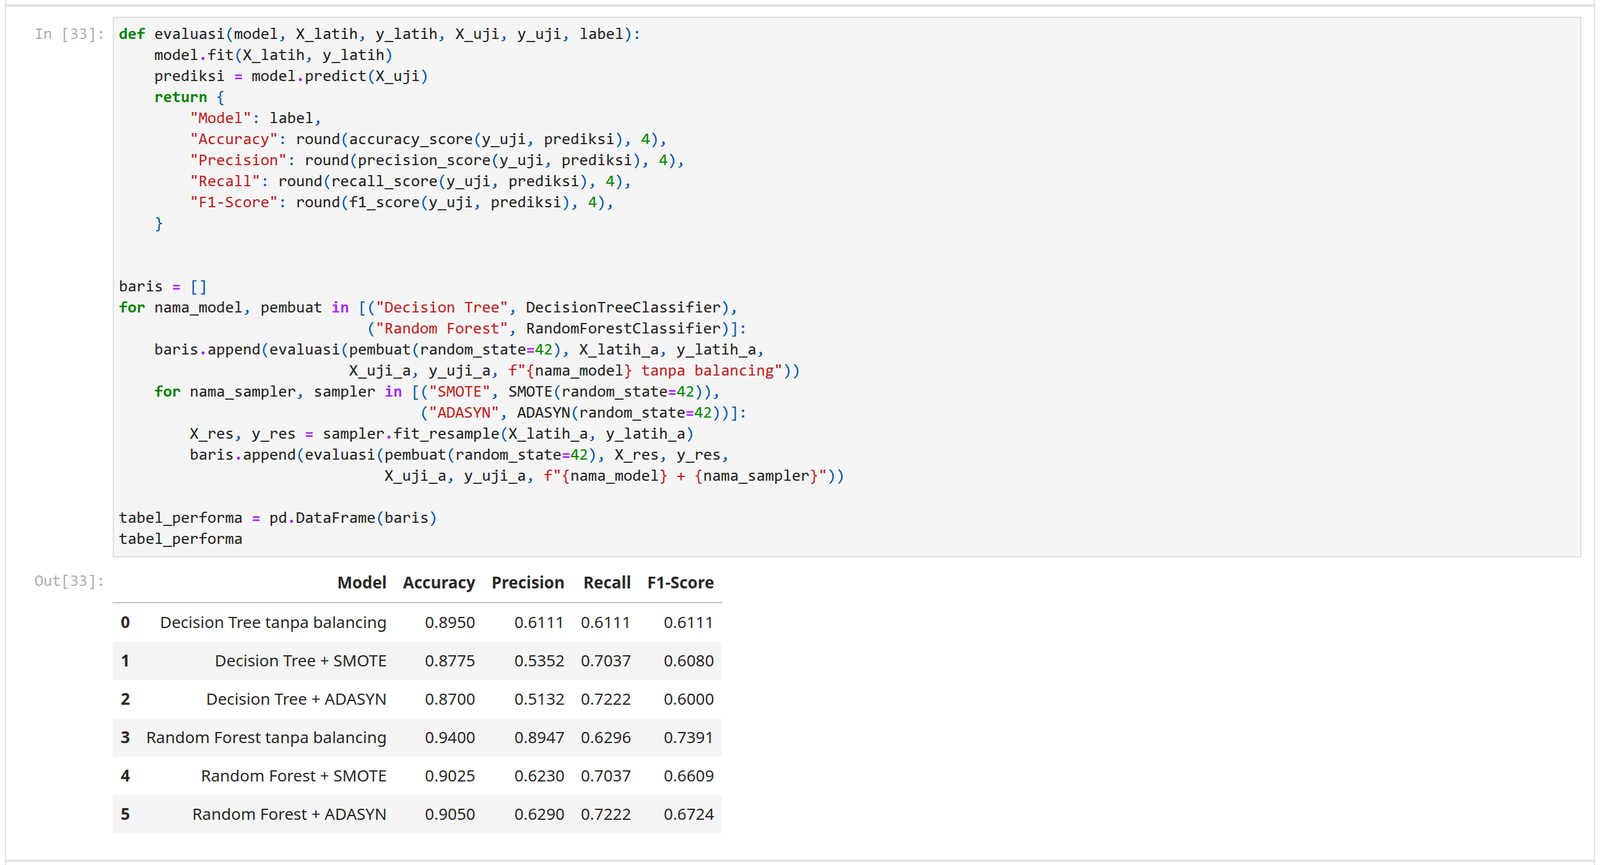
\includegraphics[width=0.95\textwidth]{images/ss-31-tugas2-tabel-performa.png}
\caption{Tangkapan layar tabel performa dua pengklasifikasi pada tiga kondisi penyeimbangan.}
\label{fig:ss-tabel-performa}
\end{figure}

\begin{table}[H]
\centering
\caption{Performa model sebelum dan sesudah penyeimbangan pada dataset Wine Quality.}
\label{tab:performa-wine}
\small
\begin{tabular}{|l|r|r|r|r|}
\hline
\textbf{Model} & \textbf{Accuracy} & \textbf{Precision} & \textbf{Recall} & \textbf{F1-Score} \\
\hline
Decision Tree tanpa balancing & 0,8950 & 0,6111 & 0,6111 & 0,6111 \\
\hline
Decision Tree + SMOTE & 0,8775 & 0,5352 & 0,7037 & 0,6080 \\
\hline
Decision Tree + ADASYN & 0,8700 & 0,5132 & 0,7222 & 0,6000 \\
\hline
Random Forest tanpa balancing & 0,9400 & 0,8947 & 0,6296 & 0,7391 \\
\hline
Random Forest + SMOTE & 0,9025 & 0,6230 & 0,7037 & 0,6609 \\
\hline
Random Forest + ADASYN & 0,9050 & 0,6290 & 0,7222 & 0,6724 \\
\hline
\end{tabular}
\end{table}

\begin{figure}[H]
\centering
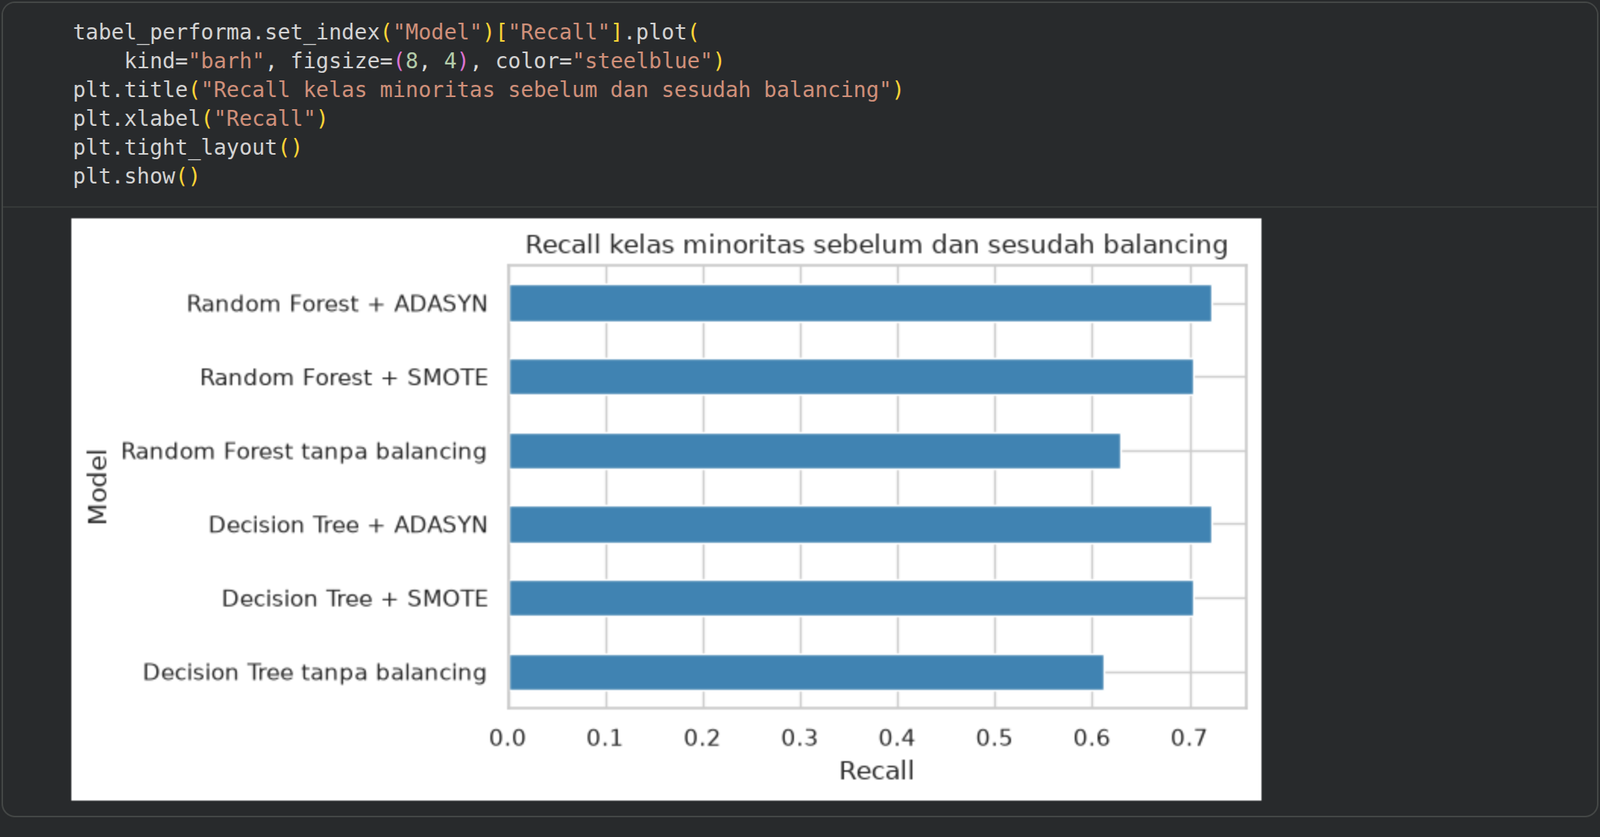
\includegraphics[width=0.75\textwidth]{images/ss-32-tugas2-recall.png}
\caption{Perbandingan \textit{recall} kelas minoritas pada enam konfigurasi model.}
\label{fig:ss-recall}
\end{figure}

Polanya konsisten pada kedua pengklasifikasi. Akurasi turun, \textit{recall} naik. Pada \textit{Decision Tree}, akurasi bergerak dari 0,8950 ke 0,8775 (SMOTE) dan 0,8700 (ADASYN), sementara \textit{recall} naik dari 0,6111 ke 0,7037 dan 0,7222. Pada \textit{Random Forest}, akurasi turun dari 0,9400 ke 0,9025 dan 0,9050, sedangkan \textit{recall} naik dari 0,6296 ke 0,7037 dan 0,7222.

Penurunan akurasi adalah konsekuensi yang diharapkan dari pergeseran titik operasi ini. Model yang lebih jarang melewatkan sampel premium memang harus menerima lebih banyak tebakan salah pada kelas standar, dan itulah harga yang dibayar untuk menaikkan \textit{recall} sekitar 9 sampai 11 poin persen. Pada konteks penyaringan kualitas, melewatkan anggur premium yang sebenarnya laku mahal biasanya lebih merugikan dibanding salah menaikkan satu produk standar ke kategori premium.

Perubahan \textit{precision} menjelaskan mekanismenya. Nilai \textit{precision} turun cukup tajam, dari 0,8947 menjadi 0,6230 pada \textit{Random Forest}. Model jadi lebih agresif menyatakan sebuah sampel premium, sehingga sebagian prediksi positif ternyata keliru. F1-Score sebagai rata-rata harmonik keduanya ikut turun karena penurunan \textit{precision} lebih besar daripada kenaikan \textit{recall}. Penyeimbangan memindahkan titik operasi model ke arah sensitivitas, dan pemilihan teknik tetap harus mempertimbangkan biaya kesalahan di domain yang dihadapi. ADASYN sedikit lebih unggul dibanding SMOTE pada \textit{recall} di kedua model, yaitu 0,7222 berbanding 0,7037. Selisihnya berasal dari cara ADASYN memusatkan sampel sintetis di sekitar batas keputusan. Namun keunggulan itu diikuti \textit{precision} yang lebih rendah, sehingga F1-Score keduanya hampir setara.

\clearpage

\chapter{Kesimpulan}
Berdasarkan praktikum yang telah saya laksanakan pada Pertemuan 7, diperoleh kesimpulan sebagai berikut:
\begin{enumerate}[noitemsep, topsep=2pt, parsep=0pt, partopsep=0pt]
    \item \textit{Imbalanced class} membuat model bias ke kelas mayoritas. Pada \textit{Stroke Prediction Dataset}, rasio kelas mencapai 19,52 banding 1 dengan hanya 4,87\% pasien mengalami stroke, sehingga akurasi menjadi metrik yang menyesatkan dan \textit{recall} kelas minoritas lebih layak dijadikan acuan.
    \item Empat teknik penyeimbangan menghasilkan karakter data yang berbeda meski tujuannya sama. \textit{Random Under-Sampling} memangkas set pelatihan dari 3.832 menjadi 338 baris dan membuang 95,4\% sampel mayoritas. \textit{Random Over-Sampling}, SMOTE, dan ADASYN sama-sama menaikkan jumlah sampel minoritas menjadi sekitar 3.663, tetapi hanya SMOTE dan ADASYN yang menambah variasi karena datanya sintetis.
    \item ADASYN membangkitkan 3.507 sampel sintetis dan berakhir dengan 3.676 sampel minoritas, tiga belas lebih banyak dari kelas mayoritas. Kelebihan itu muncul karena kuota sintetis dibagi menurut bobot kesulitan tiap sampel, bukan dibagi rata.
    \item Penyeimbangan hanya boleh diterapkan pada set pelatihan. Menerapkannya pada set pengujian akan membuat evaluasi kehilangan makna karena data uji tidak lagi mencerminkan sebaran asli.
    \item Seleksi fitur menaikkan akurasi uji \textit{Decision Tree} pada dataset heart dari 0,754 menjadi 0,820, atau 6,6 poin persen. \textit{Wrapper} RFE mencapai hasil tertinggi dengan lima fitur saja, sehingga paling efisien di antara ketiga pendekatan.
    \item \textit{Filter} ANOVA dan \textit{embedded} ExtraTree memilih himpunan fitur yang hampir sama, yaitu \texttt{caa}, \texttt{cp}, \texttt{exng}, \texttt{thall}, \texttt{oldpeak}, dan \texttt{thalachh}. Keduanya menilai kemampuan fitur memisahkan kelas, hanya metriknya berbeda.
    \item \textit{Overfitting} terlihat dari jarak akurasi latih dan uji. Pohon penuh mencapai 0,996 pada data latih tetapi hanya 0,770 pada data uji. Pemangkasan kedalaman menjadi 3 menurunkan akurasi latih ke 0,843 dan menaikkan akurasi uji ke 0,787, sehingga jaraknya menyempit dari 0,226 menjadi 0,056.
    \item Pada dataset Wine Quality, penyeimbangan menaikkan \textit{recall} kelas minoritas 9 sampai 11 poin persen tetapi menurunkan akurasi 2 sampai 3,5 poin persen.
\end{enumerate}

\clearpage

\addcontentsline{toc}{chapter}{Daftar Pustaka}
\renewcommand{\bibname}{Daftar Pustaka}
\begin{thebibliography}{99}
    \bibitem{istiana2023} A. Istiana and M. Mustafiril, ``Perbandingan Metode Klasifikasi pada Data dengan Imbalance Class dan Missing Value,'' \textit{JURNAL INFORMATIKA}, pp. 101--108, 2023.

    \bibitem{normawati2021} Normawati and T. Prayogi, ``Implementasi Naïve Bayes Classifier dan Confusion Matrix pada Analisis Sentimen Berbasis Teks pada Twitter,'' \textit{J-SAKTI (Jurnal Sains Komputer \& Informatika)}, pp. 697--711, 2021.

    \bibitem{septiana2021} R. Septiana, A. Susanto, and Tukiyat, ``Analisis Sentimen Vaksinasi Covid-19 pada Twitter Menggunakan Naive Bayes Classifier dengan Feature Selection Chi-Squared Statistic dan Particle Swarm Optimization,'' \textit{Jurnal Sistem Komputer dan Kecerdasan Buatan}, pp. 49--56, 2021.

    \bibitem{pratama2023} R. Pratama and K. Kusnawi, ``Komparasi Algoritma Supervised Learning dan Feature Selection pada Klasifikasi Penyakit Gagal Jantung,'' \textit{Indonesian Journal of Computer Science}, pp. 3722--3733, 2023.

    \bibitem{guyon2003} I. Guyon and A. Elisseeff, ``An Introduction to Variable and Feature Selection,'' \textit{Journal of Machine Learning Research}, vol. 3, pp. 1157--1182, 2003. [Online]. Tersedia: \url{https://www.jmlr.org/papers/v3/guyon03a.html}.

    \bibitem{kohavi1997} R. Kohavi and G. H. John, ``Wrappers for Feature Subset Selection,'' \textit{Artificial Intelligence}, vol. 97, no. 1--2, pp. 273--324, 1997. [Online]. Tersedia: \url{https://doi.org/10.1016/S0004-3702(97)00043-X}.

    \bibitem{guyon2002} I. Guyon, J. Weston, S. Barnhill, and V. Vapnik, ``Gene Selection for Cancer Classification Using Support Vector Machines,'' \textit{Machine Learning}, vol. 46, no. 1, pp. 389--422, 2002. [Online]. Tersedia: \url{https://doi.org/10.1023/A:1012487302797}.

    \bibitem{tibshirani1996} R. Tibshirani, ``Regression Shrinkage and Selection via the Lasso,'' \textit{Journal of the Royal Statistical Society: Series B (Methodological)}, vol. 58, no. 1, pp. 267--288, 1996.

    \bibitem{breiman2001} L. Breiman, ``Random Forests,'' \textit{Machine Learning}, vol. 45, no. 1, pp. 5--32, 2001. [Online]. Tersedia: \url{https://doi.org/10.1023/A:1010933404324}.

    \bibitem{chawla2002} N. V. Chawla, K. W. Bowyer, L. O. Hall, and W. P. Kegelmeyer, ``SMOTE: Synthetic Minority Over-sampling Technique,'' \textit{Journal of Artificial Intelligence Research}, vol. 16, pp. 321--357, 2002. [Online]. Tersedia: \url{https://doi.org/10.1613/jair.953}.

    \bibitem{he2008} H. He, Y. Bai, E. A. Garcia, and S. Li, ``ADASYN: Adaptive Synthetic Sampling Approach for Imbalanced Learning,'' in \textit{IEEE International Joint Conference on Neural Networks (IJCNN)}, pp. 1322--1328, 2008. [Online]. Tersedia: \url{https://web.archive.org/web/2024/https://doi.org/10.1109/IJCNN.2008.4633969}.

    \bibitem{wijayanti2021} N. L. P. Wijayanti, I. W. Kencana, and I. M. Sumarjaya, ``SMOTE: Potensi dan Kekurangannya pada Survei,'' \textit{E-Jurnal Matematika}, pp. 235--240, 2021.

    \bibitem{ramadhanti2022} A. P. Ramadhanti, H. B. Santoso, and T. Widiharih, ``Perbandingan SMOTE dan ADASYN pada Data Imbalance untuk Klasifikasi Rumah Tangga Miskin Kabupaten Temanggung dengan Algoritma K-Nearest Neighbor,'' \textit{JURNAL GAUSSIAN}, pp. 499--505, 2022.

    \bibitem{lemaitre2017} G. Lemaître, F. Nogueira, and C. K. Aridas, ``Imbalanced-learn: A Python Toolbox to Tackle the Curse of Imbalanced Datasets in Machine Learning,'' \textit{Journal of Machine Learning Research}, vol. 18, no. 17, pp. 1--5, 2017. [Online]. Tersedia: \url{https://jmlr.org/papers/v18/16-365.html}.

    \bibitem{pedregosa2011} F. Pedregosa \textit{et al.}, ``Scikit-learn: Machine Learning in Python,'' \textit{Journal of Machine Learning Research}, vol. 12, pp. 2825--2830, 2011. [Online]. Tersedia: \url{https://jmlr.org/papers/v12/pedregosa11a.html}.

    \bibitem{cortez2009} P. Cortez, A. Cerdeira, F. Almeida, T. Matos, and J. Reis, ``Modeling Wine Preferences by Data Mining from Physicochemical Properties,'' \textit{Decision Support Systems}, vol. 47, no. 4, pp. 547--553, 2009. [Online]. Tersedia: \url{https://doi.org/10.1016/j.dss.2009.05.016}.

    \bibitem{kaggle-stroke} Fedesoriano, ``Stroke Prediction Dataset,'' Kaggle. [Online]. Tersedia: \url{https://www.kaggle.com/datasets/fedesoriano/stroke-prediction-dataset}.

    \bibitem{kaggle-heart} R. R. Pritom, ``Heart Attack Analysis and Prediction Dataset,'' Kaggle. [Online]. Tersedia: \url{https://www.kaggle.com/datasets/rashikrahmanpritom/heart-attack-analysis-prediction-dataset}.

    \bibitem{uci-wine} P. Cortez, ``Wine Quality,'' UCI Machine Learning Repository. [Online]. Tersedia: \url{https://archive.ics.uci.edu/dataset/186/wine+quality}.

    \bibitem{sklearn-docs} Scikit-learn Developers, ``Feature Selection,'' [Online]. Tersedia: \url{https://scikit-learn.org/stable/modules/feature_selection.html}.

    \bibitem{imblearn-docs} Imbalanced-learn Developers, ``imbalanced-learn documentation,'' [Online]. Tersedia: \url{https://imbalanced-learn.org/stable/}.

    \bibitem{python-docs} Python Software Foundation, ``Python 3 Documentation,'' [Online]. Tersedia: \url{https://docs.python.org/3/}.

    \bibitem{pandas-docs} The pandas Development Team, ``pandas documentation,'' [Online]. Tersedia: \url{https://pandas.pydata.org/docs/}.

    \bibitem{numpy-docs} NumPy Developers, ``NumPy user guide,'' [Online]. Tersedia: \url{https://numpy.org/doc/stable/}.

    \bibitem{matplotlib-docs} The Matplotlib Development Team, ``Matplotlib Documentation,'' [Online]. Tersedia: \url{https://matplotlib.org/stable/contents.html}.

    \bibitem{seaborn-docs} M. Waskom, ``Seaborn: statistical data visualization,'' [Online]. Tersedia: \url{https://seaborn.pydata.org/}.

    \bibitem{colab-notebook} H. R. Prasetya, ``Praktikum 7: Imbalanced Dataset dan Feature Selection (Notebook),'' Google Colaboratory, 2026. [Online]. Tersedia: \url{https://colab.research.google.com/github/hafidzrizqullahprasetya/PPD/blob/main/pertemuan-7/praktikum-7-imbalanced-feature-selection.ipynb}.
\end{thebibliography}

\end{document}
